\chapter{Weak Galerkin Parallel Solutions of Linear Elasticity on Unstructured Meshes}

This chapter focuses on solving linear elasticity problem on parallel computer by combining a novel finite element method with an efficient parallel computing scheme. Specifically, this combination involves a discontinuous weak Galerkin finite element method \cite{mu2012weak, li2013weak, wang2014weak, mu2013computational} and a non-overlapping domain decomposition scheme, namely, the balancing domain decomposition with constraints (BDDC) \cite{dohrmann2003preconditioner,tu2007three2d,tu2007three3d}. The WG method is considered as a newly developed robust numerical method and inherits the locking-free feature for the linear elastic equation \cite{wang2016locking}. 

Like the standard Finite Element method (FEM), the WG method can be used to solve generic partial differential equations. An advanced feature of the WG finite element method is that the entire problem is decomposed into multiple elemental problems. Such elemental problems are often derived from weak formulations of the corresponding differential operators after integration by parts. In these elemental problems, the differential operators are approximated and reconstructed by smaller-size matrices. The WG method has been proven robust and possessing optimal orders of accuracy in spatial discretization on serial computers \cite{mu2014weak, Mu2015new}. Wang et al \cite{wang2016locking} recently extended the WG method to solve linear elasticity problems and also successfully demonstrated its locking-free property. However, the performance of the WG method on parallel computers has not yet been examined. In this chapter, we design and develop the WG-BDDC scheme to bring the WG method to solve engineering problem in parallel fashion. This is the first attempt in our knowledge. The successful results indicate that it's a promising direction to develop an efficient and parallel structural solver.



\section{Domain Decomposition Scheme}
The basic idea of domain decomposition is to split the computational mesh of an entire domain into many smaller meshes for a set of non-overlapping subdomains. Each subdomain contains its own set of grid elements. For finite element methods, after domain decomposition, a remaining challenging task is to connect these subdomains' interfaces by satisfying continuity constraints to correctly represent the solution of the original set of equations over the complete domain. In this work, the BDDC method is used to serve this purpose. The original balancing domain decomposition (BDD) method \cite{mandel1993balancing} has only considered two level meshes. It used a multiplicative coarse domain to correct the local fine mesh subdomain. However, the significant difference between BDDC and BDD is that the method in this paper applies the coarse problem in an additive routine rather than multiplicative manner. In this case, a more flexible of constraints will reduce the complexity and improve the efficiency. In our BDDC method, we assemble the preconditioner matrix additively in contrast to the multiplicative coarse grid correction used in the BDD method. In the BDDC method, the flexibility of choosing constraining points leads to reduced complexity of implementation and improved efficiency of computations in comparison to the standard BDD method. The details of the choice of constraints for BDDC will be discussed in this section.

\subsection{FETI-DP Method}
Finite Element Tearing and Interconnect (FETI) , first proposed by Farhat \cite{farhat1991method, farhat1994optimal, klawonn2001feti, farhat1998two, li2006feti, klawonn2006dual}, is a popular method for solving large finite element problems. Originally, FETI is proposed to solve the discontinuity when applying domain decomposition on second order elliptic partial differential equations, particularly  elasticity equations. FETI method partitioned the entire computational domain into two level meshes, the coarse grid and fine grid. Lagrangian multiplier is employed to resolve the singularity for the matrix of every subdomain after the domain decomposition. For the fine mesh, since local matrix is not positive definite, the pseudo-inverse is applied to invert the local matrix. Combining the Lagrangian multiplier and pseudo-inverse, FETI method bypass the rigid body motion problem and partitioned the continuous problem to multiple non-overlapping subdomains.

Then FETI-DP (Dual Primal) is introduced for two-dimensional problems by Farhat and Rixen \cite{farhat2001feti}. In this method, the unknown variables on the interface is partitioned into primal and dual spaces. The continuity of the primal unknown variables along the interface, the vertices of each subdomain, is maintained by assemblage. For the dual space, the constraints are represented by Lagrange multipliers. 

In this section, we begin with an example of a two-dimensional, two partitioned subdomain case. The unknown variables $ \mathbf{u} $ are represented by the solid squares on the interface. We enforce the Dirichlet boundary condition on the boundary. The original geometry and computational domain is  

\begin{figure}[h]
	\centering
	\begin{tabular}{c}
		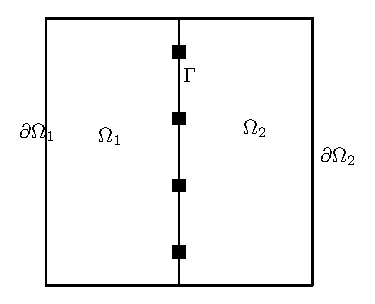
\includegraphics[width=0.6\textwidth]{./pics/feti1}
	\end{tabular}
	\caption{\footnotesize Computational domain partitioned into two nonoverlapping subdomains.}\label{fig4: feti1}
\end{figure}

the original governing equation in matrix form is $ \mathbf{A} \mathbf{u} = \mathbf{f} $. We begin to compute the stiffness matrix for each subdomain that

\begin{equation}
 \begin{pmatrix}
A_{II}^{(j)} & A_{I\Gamma}^{(j)} \\
A_{\Gamma I}^{(j)} & A_{\Gamma \Gamma}^{(j)}
\end{pmatrix} \begin{pmatrix}
u_{I}^{(j)} \\ u_{\Gamma}^{(j)}
\end{pmatrix} = \begin{pmatrix}
f_{I}^{(j)} \\ f_{\Gamma}^{(j)}
\end{pmatrix}
\end{equation}
where $ j = 1, 2 $.


The boundary condition along $ \partial \Omega  $ is Dirichlet condition, a homogeneous Neumann condition is applied on $ \Gamma $.

The global problem after assemblage is that
\begin{equation}
\begin{pmatrix}
A_{II}^{(1)} & 0 & A_{I\Gamma}^{(1)} \\
0 & A_{II}^{(2)} & A_{I\Gamma}^{(2)} \\
A_{\Gamma I}^{(1)} & A_{\Gamma I}^{(2)} & A_{\Gamma \Gamma}\\
\end{pmatrix} \begin{pmatrix}
u_{I}^{(1)} \\ u_{I}^{(2)} \\ u_{\Gamma}
\end{pmatrix} = \begin{pmatrix}
f_{I}^{(1)} \\ f_{I}^{(2)} \\ f_{\Gamma}
\end{pmatrix}
\end{equation}
where $ A_{\Gamma} = A_{\Gamma \Gamma}^{(1)} + A_{\Gamma \Gamma}^{(2)} $ and $ f_{\Gamma} = f_{\Gamma}^{(1)} + f_{\Gamma}^{(2)} $. The unknown variables are decomposed into two computational subdomains. The degree of freedoms are represented by $ u_{I}^{(1)} $, $ u_{I}^{2} $ and $ u_{\Gamma} $ corresponding to the domains $ \Omega_{1}, \Omega_{2} $ and $ \Gamma $ respectively.

Since the interior matrices are square and can be inverted. Then we can eliminate the interior unknown variables by Schur complement operators. The interface unknown DOFs shall have the new form as
\begin{equation}
S^{(j)} := A_{\Gamma \Gamma}^{(j)} - A_{\Gamma I}^{(j)} {A_{II}^{(j)}}^{-1}A_{I \Gamma}^{(j)}
\end{equation}

\begin{equation}
g_{\Gamma}^{(j)} := f_{\Gamma}^{(j)} - A_{\Gamma I}^{(j)} {A_{II}^{(i)}}^{-1} f_{I}^{(j)}
\end{equation}

based on the given matrix $ Au = f $, we can reduce the equation matrices into interface DOF only system

\begin{equation}
(S^{(1)} + S^{(2)}) u_{\Gamma} = g_{\Gamma}^{(1)} + g_{\Gamma}^{2}
\end{equation}

After the Schur complement, the original global matrix $ A $ is reduced the unknown variables on the interface only $ g_{\Gamma} $. The major cost of local matrix inversion has been distributed to each local processors. The local unknown variables can be recovered locally with the solution of interface.

For FETI method, we introduce the Lagrange multiplier to enforce the continuity along the interface. The governing equation in matrix form is 
\begin{equation}
\begin{pmatrix}
A_{II}^{(j)} & A_{I \Gamma}^{(j)} \\
A_{\Gamma I}^{(j)} & A_{\Gamma \Gamma}^{(j)} \\
\end{pmatrix} \begin{pmatrix}
u_{I}^{(j)} \\ u_{\Gamma}^{(j)} 
\end{pmatrix} = \begin{pmatrix}
f_{I}^{(j)} \\ f_{\Gamma}^{(j)} + \lambda_{\Gamma}^{(j)}
\end{pmatrix}
\end{equation}
where $ j = 1, 2 $ and $ \lambda_{\Gamma} = \lambda_{\Gamma}^{(1)} = - \lambda_{\Gamma}^{(2)} $. $ \lambda_{\Gamma} $ is an unknown flux vector, namely, Lagrange multiplier. We can solve this linear system following Eq. (4.3) to Eq. (4.5)

\begin{equation}
g_{\Gamma}^{(j)} = f_{\Gamma}^{(j)} - A_{\Gamma I}^{(j)} {A_{II}^{(j)}}^{-1} f_{I}^{(j)}
\end{equation}

\begin{equation}
u_{\Gamma}^{(j)} = {S^{(j)}}^{-1} (g_{\Gamma}^{(j)} + \lambda_{\Gamma}^{(j)})
\end{equation}

The interface condition between adjacent subdomains is
\begin{equation}
u_{\Gamma}^{(1)} = u_{\Gamma}^{(2)}
\end{equation}
the value of DOFs for the same position has to be same. To resolve the rigid body motion problem, we obtain
\begin{equation}
F \lambda_{\Gamma} = d_{\Gamma}
\end{equation}
\begin{equation}
F = {S^{(1)}}^{-1} + {S^{(2)}}^{-1}
\end{equation}

An improved version of FETI is FETI-DP. We further divide the interface to primal and dual spaces,

\begin{figure}[h]
	\centering
	\begin{tabular}{c}
		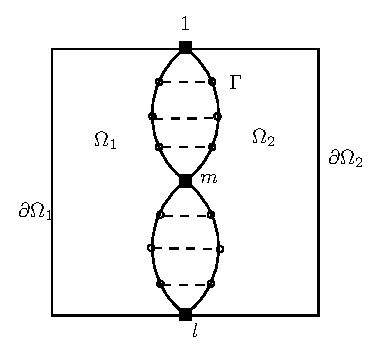
\includegraphics[width=0.5\textwidth]{./pics/feti2}
	\end{tabular}
	\caption{\footnotesize Computational domain partitioned into two nonoverlapping subdomains with floating constaint.}
\end{figure}

From the Fig 4.2, the interface edge is continued to split into $ (u_1, \cdots, u_m, \cdots, u+l) $. The solid squares represent the unknown variables belong to primal space, the hollow dots represent the unknown variables belong to the dual space. The original interface is partially teared. The curve and dots mean the new local unknown variables after the tearing. The connecting squares represent the reconnecting. This graph shows the origin of the name of FETI-DP. The linear system can be written as

\begin{equation}
\begin{pmatrix}
A_{II}^{(j)} & A_{1I}^{(j)} & \cdots & A_{mI}^{(j)} & \cdots & A_{l I}^{(j)} \\
A_{1 I}^{(j)} & A_{11}^{(j)} & \cdots & A_{1m}^{(j)} & \cdots & A_{1l}^{(j)} \\
\vdots & \vdots & \ddots & \vdots & \ddots & \vdots \\
A_{mI}^{(j)} & A_{m1}^{(j)} & \cdots & A_{mm}^{(j)} & \cdots & A_{ml}^{(j)} \\
\vdots & \vdots & \ddots & \vdots & \ddots & \vdots \\
A_{lI}^{(j)} & A_{l1}^{(j)} & \cdots & A_{lm}^{(j)} & \cdots & A_{ll}^{(j)}\\
\end{pmatrix} \begin{pmatrix}
u_{I}^{(j)} \\ u_{1}^{(j)} \\ \vdots \\ u_{m}^{(j)} \\ \vdots \\ u_{l}^{(j)}\\
\end{pmatrix} = \begin{pmatrix}
f_{I}^{(j)} \\ f_{1}^{(j)} \\ \vdots \\ f_{m}^{(j)} \\ \vdots \\ f_{l}^{(j)}
\end{pmatrix}
\end{equation}

The variables along the interface between the two nonoverlapping subdomians can be written as
\begin{equation}
\begin{pmatrix}
u_{1}^{(j)} \\ \vdots \\ u_{m}^{(j)} \\ \vdots \\ u_{l}^{(j)}
\end{pmatrix} = T_{E} \begin{pmatrix}
\hat{u}_{1}^{(j)} \\ \vdots \\ \hat{u}_{m}^{(j)} \\ \vdots \\ \hat{u}_{l}^{(j)}
\end{pmatrix} = \begin{pmatrix}
1 & \cdots & 1 & 0 & \cdots \\
\vdots & \ddots & \vdots & 0 & \cdots \\
-1 & \cdots & 1 & \cdots & -1 \\
\cdots & 0 & \vdots & \ddots &  \vdots \\
\cdots & 0 & 1 & \cdots & 1\\
\end{pmatrix} \begin{pmatrix}
\hat{u}_{1}^{(j)} \\ \vdots \\ \hat{u}_{m}^{(j)} \\ \vdots \\ \hat{u}_{l}^{(j)}
\end{pmatrix}
\end{equation}

After the multiplication between vector and matrix we have
\begin{equation}
T_{E} \begin{pmatrix}
\hat{u}_{1}^{(j)} \\ \vdots \\ \hat{u}_{m}^{(j)} \\ \vdots \\ \hat{u}_{l}^{(j)}
\end{pmatrix} = \begin{pmatrix}
1 \\ \vdots \\ 1 \\ \vdots \\ 1
\end{pmatrix} \hat{u}_{m}^{(j)} + \begin{pmatrix}
& & \hat{u}_{1}^{(j)} & & \\
& & \vdots & & \\
-\hat{u}_{1}^{(j)} & -\cdots & -\hat{u}_{m-1}^{(j)} & \hat{u}_{m+1}^{(j)} & -\hat{u}_{l}^{(j)}\\
& & \vdots & & \\
& & \hat{u}_{l}^{(j)} & & \\
\end{pmatrix}
\end{equation}
the $ T_{E} $ is a square matrix and each columns represents the new space of interface unknown variables. The original interface is divided into two spaces. One is the local space and another is the interface space. The the problem can be written as

\begin{equation}
T^{T} \begin{pmatrix}
A_{II}^{(j)} & A_{1I}^{(j)} & \cdots & A_{mI}^{(j)} & \cdots & A_{l I}^{(j)} \\
A_{1 I}^{(j)} & A_{11}^{(j)} & \cdots & A_{1m}^{(j)} & \cdots & A_{1l}^{(j)} \\
\vdots & \vdots & \ddots & \vdots & \ddots & \vdots \\
A_{mI}^{(j)} & A_{m1}^{(j)} & \cdots & A_{mm}^{(j)} & \cdots & A_{ml}^{(j)} \\
\vdots & \vdots & \ddots & \vdots & \ddots & \vdots \\
A_{lI}^{(j)} & A_{l1}^{(j)} & \cdots & A_{lm}^{(j)} & \cdots & A_{ll}^{(j)}\\
\end{pmatrix} T \begin{pmatrix}
u_{I}^{(j)} \\ \hat{u}_{1}^{(j)} \\ \vdots \\ \hat{u}_{m}^{(j)} \\ \vdots \\ \hat{u}_{l}^{(j)}\\
\end{pmatrix} = T^{T} \begin{pmatrix}
f_{I}^{(j)} \\ f_{1}^{(j)} \\ \vdots \\ f_{m}^{(j)} \\ \vdots \\ f_{l}^{(j)}
\end{pmatrix}
\end{equation}

same as previous equation, $ T $ is a diagonal block matrix 
\begin{equation}
T = \begin{pmatrix}
I & 0 \\ 
0 & T_{E}\\
\end{pmatrix}
\end{equation}

 We can assume that the unknown variables on each subdomain have been changed when using primal space. We can see that the primal space is the only connection along the interface. The other DOFs are in dual space including interior unknowns and the rest interface nodes.

\begin{equation}
\begin{pmatrix}
A_{II}^{(1)} &  A_{\Delta I}^{(1)}& 0 & 0 & A_{\Pi I}^{(1)} & 0 \\
A_{\Delta I}^{(1)} & A_{\Delta \Delta}^{(1)} & 0 & 0& A_{\Pi \Delta}^{(1)} & B_{\Delta}^{(1)}\\
0 & 0 & A_{II}^{(2)} & A_{\Delta I}^{(2)} & A_{\Pi I}^{(2)} & 0 \\
0 & 0 & A_{\Delta I}^{(2)} & A_{\Delta \Delta}^{(2)} & A_{\Pi \Delta}^{(2)} & B_{\Delta}^{(2)} \\
A_{\Pi I}^{(1)} & A_{\Pi \Delta}^{(1)} & A_{\Pi I}^{(2)} & A_{\Pi \Delta}^{(2)} & A_{\Pi \Pi}^{(1)} + A_{\Pi \Pi}^{(2)} & 0 \\
0 & B_{\Delta}^{(1)} & 0 & B_{\Delta}^{(2)} & 0 & 0 \\
\end{pmatrix} \begin{pmatrix}
u_{I}^{(1)} \\ u_{\Delta}^{(1)} \\ u_{I}^{(2)} \\ u_{\Delta}^{(2)} \\ u_{\Pi} \\ \lambda\\
\end{pmatrix} = \begin{pmatrix}
f_{I}^{(1)} \\ f_{\Delta}^{(1)} \\ f_{I}^{(2)} \\ f_{\Delta}^{(2)} \\ f_{\Pi}^{(1)} + f_{\Pi}^{(2)} \\ 0\\
\end{pmatrix}
\end{equation}

We can further eliminate the local variables $ u_{I}^{(1)}, u_{\Delta}^{(1)}, u_{I}^{(2)} $ and $ u_{\Delta}^{(2)} $, so that we can obtain
\begin{equation}
\begin{pmatrix}
S_{\Pi \Pi} & \tilde{B}_{\Lambda \Pi}^{T} \\ 
\tilde{B}_{\Lambda \Pi} & \tilde{B}_{\Lambda \Lambda} \\
\end{pmatrix} \begin{pmatrix}
u_{\Pi} \\ \lambda \\
\end{pmatrix} = \begin{pmatrix}
g_{\Pi} \\ d_{\Lambda}\\
\end{pmatrix}
\end{equation}

the details of above equation is 

\begin{equation}
S_{\Pi \Pi} = \sum_{j = 1}^{2} R_{\Pi}^{(j)} \begin{pmatrix}
A_{\Pi \Pi}^{(j)} - \begin{bmatrix}
A_{\Pi I}^{(j)} & A_{\Pi \Delta}^{(j)} \\
\end{bmatrix} \begin{bmatrix}
A_{II}^{(j)} & A_{I \Delta}^{(j)} \\
A_{\Delta I}^{(j)} & A_{\Delta \Delta}^{(j)}
\end{bmatrix}^{-1} \begin{bmatrix}
A_{\Pi I}^{(j)} \\ A_{\Pi \Delta}^{(j)} \\
\end{bmatrix}
\end{pmatrix} R_{\Pi}^{(j)} ,
\end{equation}

\begin{equation}
\tilde{B}_{\Lambda \Pi} = - \sum_{j = 1}^{2} \begin{bmatrix}
0 & B_{\Pi}^{(j)}
\end{bmatrix} \begin{bmatrix}
A_{II}^{(j)} & A_{\Delta I}^{(j)} \\
A_{\Delta I}^{(j)} & A_{\Delta \Delta}^{(j)}
\end{bmatrix}^{-1} \begin{bmatrix}
A_{\Pi I}^{(j)} \\ A_{\Pi \Delta}^{(j)}
\end{bmatrix} R_{\Pi}^{(j)} ,
\end{equation}

\begin{equation}
\tilde{B}_{\Lambda \Lambda} = - \sum_{j = 1}^{2} \begin{bmatrix}
0 & B_{\Delta}^{(j)}
\end{bmatrix} \begin{bmatrix}
A_{II}^{(j)} & A_{\Delta I}^{(j)} \\
A_{\Delta I}^{(j)} & A_{\Delta \Delta}^{(j)}
\end{bmatrix}^{-1} \begin{bmatrix}
0 \\B_{\Delta}^{(j)} \\
\end{bmatrix} ,
\end{equation}

\begin{equation}
g_{\Pi} = \sum_{j = 1}^{2} R_{\Pi}^{(j)} \begin{pmatrix}
f_{\Pi}^{(j)} - \begin{bmatrix}
A_{\Pi I}^{(j)} & A_{\Pi \Delta}^{(j)}
\end{bmatrix} \begin{bmatrix}
A_{II}^{(j)} & A_{\Pi \Delta}^{(j)} \\
\end{bmatrix} \begin{bmatrix}
A_{II}^{(j)} & A_{\Delta I}^{(j)} \\
A_{\Delta I}^{(j)} & A_{\Delta \Delta}^{(j)}\\
\end{bmatrix}^{-1} \begin{bmatrix}
f_{I}^{(j)} \\ f_{\Delta}^{(j)}
\end{bmatrix}
\end{pmatrix} ,
\end{equation}

\begin{equation}
d_{\Lambda} = - \sum_{j = 1}^{2} \begin{bmatrix}
0 & B_{\Delta}^{(j)} \\
\end{bmatrix} \begin{bmatrix}
A_{II}^{(j)} & A_{\Delta I}^{(j)} \\
A_{\Delta I}^{(j)} & A_{\Delta \Delta}^{(j)} 
\end{bmatrix}^{-1} \begin{bmatrix}
f_{I}^{(j)} \\ f_{\Delta}^{(j)} \\
\end{bmatrix}
\end{equation}

whre the $ R_{\Pi}^{(j)} $ is a projection matrix that mapping the local subdomain element to global elements with $ \{0, 1\} $ values. In this example, both projection values are equal to $ 1 $.

For the linear system, the Lagrange multiplier $ \lambda $ is
\begin{equation}
\begin{pmatrix}
\tilde{B}_{\Lambda \Lambda} - \tilde{B}_{\Lambda \Pi} S_{\Pi \Pi}^{-1} \tilde{B}_{\Lambda \Pi}^{T}
\end{pmatrix} \lambda = d_{\Lambda} - \tilde{B}_{\Lambda \Pi} S_{\Pi \Pi}^{-1} g_{\Pi}
\end{equation}

A Dirichlet preconditioner is applied in FETI-DP method for solving above equation. 

Based on above linear system, Lagrange multiplier is an external unknown vector $ \lambda $ and requires lots of computational effort to assemble the matrix. When we try to solve the such a linear system, it's common to obtain the result along the dual space that $ u_{\Delta}^{(1)} \neq  u_{\Delta}^{(2)}$. To maintain the continuity, we shall balance the computational cost for solving the unknown vectors. Therefore, an assembled residual of resulting vector is needed. The residue is mapped into the appropriate space of enforced vector on the right-hand side of the equation. Then we can use the residue vector to correct the solution and gradually obtain the final results. An improved algorithm, BDDC method, will be discussed in the following section.

\subsection{Block Cholesky elimination}

First, we consider how to represent the inverse of a matrix $ M $, which is symmetric and positive definite block matrix as

\begin{equation}\label{eq:linearSys}
M = \begin{bmatrix}
A & B^{T} \\
B & C\\
\end{bmatrix}
\end{equation}
where $ M $ is the global stiffness matrix, $ A $ is the square matrix represents the interior values of each subdomain, $ C $ is the values on the interface and $ B $ represents the connectivity between $ A $ and $ C $.

We employ the block Cholesky elimination and obtain the following equation that
\begin{equation}\label{eq:schur1}
\begin{bmatrix}
A & B^{T} \\ B & C \\
\end{bmatrix} = 
\begin{bmatrix}
I_{A} & 0 \\ BA^{-1} & I_{C}\\
\end{bmatrix} \begin{bmatrix}
A & 0 \\ 0 & C - BA^{-1} B^{T}
\end{bmatrix}
\begin{bmatrix}
I_{A} & A^{-1} B^{T} \\ 0 & I_{C} \\
\end{bmatrix}
\end{equation}

Both $ I_{A} $ and $ I_{C} $ are identity matrices. The Schur complement is represented as
\begin{equation}
\mathit{S} = C - BA^{-1} B^{T}
\end{equation}

the $ S $ can be seen as a smaller global matrix containing the information among $ A $, $ B $ and $ C $. A Schur complement matrix $ S $ , represents a smaller global stiffness matrix partially assembled by each individual subdomains. However, after the decomposition, the size of $ S $ is still too large to be directly inversed. Consequently, we introduce the primal and dual spaces to calculate a preconditioner in parallel fashion to distribute the computational load and accelerate the overall speed. We redefine the Schur complement matrix $ S $ and compute the preconditioner $ S_{BDDC} $ by a parallel fashion. The number of primal variables, the constraints through the interface, is much less than the size of Schur complement matrix.

The inverse of original matrix $ M $ is 
\begin{eqnarray} \label{eq:schur}
M^{-1} &=& \begin{bmatrix}
A & B^{T} \\
B & C\\
\end{bmatrix}^{-1} =
\begin{bmatrix}
I_{A} &  -A^{-1}B^{T} \\ 0 & I_{C}\\
\end{bmatrix} \begin{bmatrix}
A^{-1}& 0 \\ 0 & S^{-1}
\end{bmatrix}
\begin{bmatrix}
I_{A} & 0 \\ -BA^{-1} & I_{C} \\
\end{bmatrix}\\
&=& \begin{bmatrix}
A^{-1} & 0 \\ 0 & 0 \\
\end{bmatrix} + \Phi S^{-1} \Phi^{T}
\end{eqnarray}
where $ \Phi =\begin{bmatrix}
-A^{-1}B^{T} \\ I_{C}
\end{bmatrix} $
where $ I_{A} $ and $ I_{C} $ is diagonal matrix with same size as matrix $ A $ and $ C $ respectively.

The original inverse global matrix  is partitioned into one matrix containing $ A^{-1} $ and the other matrix associated with the $ S^{-1} $. The interface matrix $ S $ takes from adjacent local subdomains, corresponding to the degrees of freedom on the solid squares shown in Figure 4.2. 

After decomposing the original computational domain into subdomains, we  can demonstrate the effectiveness of the BDDC method in solving the governing equation
\begin{equation}
{M}\mathbf{u} = \mathbf{f}
\end{equation}


\subsection{Balancing Domain Decomposition by Constraints}

The balancing domain decomposition method was introduced by Mandel \cite{mandel2005algebraic}. The original idea of BDD method is applying a coarse correction to guarantee the convergence of residuals. The BDDC is a domain decomposition method for solving large symmetric, positive definite equations of linear systems. Comparing to BDD method, the substructure spaces and the coarse spaces are connected by the corner cell as constraints only. The main difference is that the BDDC method applies the coarse problem in an additive routine, which makes it possible to use a different bilinear form on the coarse problem. In this way, the BDDC method is considered as a simpler alternative to FETI-DP domain decomposition method \cite{li2006feti}. We only consider the corner connections of subdomain as the only constraints. Comparing with FETI-DP, BDDC method adds coarse degrees of freedom involving averages over edges and faces of elements. This improvement causes an obvious simplification through domain decomposition and matrix calculation.

After the Schur complement, the preconditioner for interface is 
\begin{equation}
\hat{S}u_{\Gamma} = \sum_{j = 1}^{N} R_{\Gamma}^{(j)} g_{\Gamma}
\end{equation}

where
\begin{equation}
\tilde{S} = \tilde{R}_{\Gamma}^{T} \tilde{S}_{\Gamma} \tilde{R}_{\Gamma}
\end{equation}

In the BDDC algorithm, a two-level Neumann-Neumann type preconditioner for solving this interface problem. In the BDDC preconditioner, the coarse grid is assembled from coarse basis functions. We can apply the minimum energy method on the subdomains to obtain primal constrains. The primal constraints maintain the continuity along the edge interface between two subdomains, as in FETI-DP algorithm. 

Dohrmann's BDDC preconditioner \cite{dohrmann2003preconditioner, dohrmann2003study, mandel2005algebraic} has the form
\begin{equation}
M_{BDDC}^{-1} = R_{D, \Gamma}^{T} T R_{D, \Gamma}
\end{equation}
for the coarse-level $ T $ is defined by 
\begin{equation}
T = \Psi (\Psi^{T} S \Psi)^{-1} \Psi^{T}
\end{equation}
the coarse level basis function vector is defined by 
\begin{equation}
\Psi = \begin{pmatrix}
\Psi^{(1)} \\ \vdots \\ \Psi^{(N)}\\
\end{pmatrix}
\end{equation}

Then the Schur complement coarse-level matrix can be written as 
\begin{equation}
\begin{pmatrix}
S^{(j)} & {C^{(j)}}^{T} \\
C^{(j)} & 0 \\
\end{pmatrix} \begin{pmatrix}
\Psi^{(j)} \\ V^{(j)} \\
\end{pmatrix} = \begin{pmatrix}
0 \\ R_{\Pi}^{(j)}\\
\end{pmatrix}
\end{equation}
 where $ C^{(j)} $ is the primal constraints of each subdomain and $ V^{(j)} $ is Lagrange multiplier vector. Since the variables are changing for each subdomain, then the Lagrange multiplier vector is no longer needed to enforce the primal continuity constraints and the new BDDC preconditioner can be designed as
 
 \begin{equation}
 M_{BDDC}^{-1} = R_{D, \Gamma}^{T} \{ R_{\Gamma \Delta}^{T} S^{-1}_{\Delta} R_{\Gamma \Delta} + \Psi (\Psi^{T} S \Psi)^{-1} \Psi^{T} \} R_{D, \Gamma}
 \end{equation}
 
 The primal space DOFs are used to enforce the continuity by restricting the operators to the dual interface space $ \Delta $. The governing matrix equation can be designed as
 \begin{equation}
 \begin{pmatrix}
 A_{II}^{(j)} & A_{\Delta I}^{(j)} & A^{(j)}_{\Pi I} \\
 A_{\Delta I}^{(j)} & A_{\Delta \Delta}^{(j)} & A_{\Pi \Delta}^{(j)} \\
 A_{\Pi I}^{(j)} & A_{\Pi \Delta}^{(j)} & A_{\Pi \Pi}^{(j)} \\
 \end{pmatrix} \begin{pmatrix}
 u_{I}^{(j)} \\ \Psi_{\Delta}^{(j)} \\ R_{\Pi}^{(j)} \\
 \end{pmatrix} = \begin{pmatrix}
 0 \\ 0 \\ S_{\Pi \Pi}^{(j)} R_{\Pi}^{(j)}
 \end{pmatrix}
 \end{equation}
 
 where
 
 \begin{equation}
 \Psi^{(j)} = \begin{pmatrix}
 \Psi_{\Delta}^{(j)} \\ R_{\Pi}^{(j)} \\
 \end{pmatrix}
 \end{equation}
 
 \begin{equation}
 \Psi^{(j)} = \begin{pmatrix}
 -\begin{pmatrix}
 0 & I_{\Delta}^{(j)} 
 \end{pmatrix} \begin{pmatrix}
 A_{II}^{(j)} & A_{I \Delta}^{(j)} \\
 A_{\Delta I}^{(j)} & A_{\Delta \Delta}^{(j)} \\
 \end{pmatrix}^{-1} \begin{pmatrix}
 A_{I \Pi}^{(j)} \\ A_{\Pi \Delta}^{(j)} \\
 \end{pmatrix} R_{\Pi}^{(j)} \\
 R_{\Pi}^{(j)}
 \end{pmatrix}
 \end{equation}
 
 and 
 \begin{equation}
 S_{\Pi \Pi}^{(j)} = A_{\Pi \Pi}^{(j)} - \begin{pmatrix}
 A_{\Pi I}^{(j)} & A_{\Pi \Delta}^{(j)} \\
 \end{pmatrix} \begin{pmatrix}
 A_{II}^{(j)} & A_{I \Delta}^{(j)} \\
 A_{\Delta I}^{(j)} & A_{\Delta \Delta}^{(j)}
 \end{pmatrix}^{-1} \begin{pmatrix}
 A_{I \Pi}^{(j)} \\ A_{\Delta \Pi}^{(j)}\\
 \end{pmatrix}
 \end{equation}
 
 the global Schur complement operator $ S_{\Pi \Pi} $ is assembled by every subdomain that
 
 \begin{equation}
 \Psi^{T} S \Psi = \sum_{j = 1}^{N} {\Psi^{(j)}}^{T} S^{(j)} \Psi^{(j)} 
 \end{equation}
 this equals to 
 \begin{equation}
 \sum_{j = 1}^{N} {R_{\Pi}^{(j)}}^{T} S_{\Pi \Pi}^{(j)} R_{\Pi}^{(j)} = S_{\Pi\Pi}
 \end{equation}
 where $ \Psi $ represents the interface vectors with distributed coarse-level variables. $ \Phi $ represents the unknown variable vectors on coarse-level.
 
 The averaging scaling vector is
 \begin{equation}
 \delta^{\dagger}_{j} (x) = 1, \quad x \in \Gamma
 \end{equation}
 
\begin{equation}
R_{D, \Gamma}^{T} \Psi = \tilde{R}_{D, \Gamma}^{T} \Phi
\end{equation}

therefore

\begin{equation}
M_{BDDC}^{-1} = R_{D, \Gamma}^{T} R_{\Gamma \Delta}^{T} S_{\Delta}^{-1} R_{\Gamma \Delta} R_{D, \Gamma} + R_{D, \Gamma}^{T} \Psi 
\begin{pmatrix}
\Psi^{T} S \Psi
\end{pmatrix}^{-1} \Psi^{T} R_{D, \Gamma}
\end{equation}

after replacing $ \Psi $ by $ \Phi $, we can derive
\begin{equation}
M_{BDDC}^{-1} = \tilde{R}_{D, \Gamma}^{T} R_{\Gamma \Delta}^{T} S_{\Delta}^{-1} R_{\Gamma \Delta} \tilde{R}_{\Delta, \Gamma} + \tilde{R}_{D, \Gamma}^{T} \Phi S_{\Pi \Pi}^{-1} \Phi^{T} \tilde{R}_{D, \Gamma}
\end{equation}

we can simplify the equation by 
\begin{equation}
M_{BDDC}^{-1} = \tilde{R}_{D,\Gamma}^{T} \tilde{S}_{\Gamma}^{-1} \tilde{R}_{D, \Gamma}
\end{equation}

the preconditioned BDDC operator is designed by 
\begin{equation}
\tilde{R}_{D, \Gamma}^{T} \tilde{S}_{\Gamma}^{-1} \tilde{R}_{D, \Gamma} \tilde{R}_{\Gamma}^{T}\tilde{S}_{\Gamma}\tilde{R}_{\Gamma}
\end{equation}

\section{WG-BDDC Method}
In this section, we discuss the details of combining WG method with BDDC method for solving elasticity equations. 
The preconditioned conjugate gradient method is adopted as the linear solver for BDDC method. The construction of preconditioner is crucial in the problem. The BDDC preconditioner combines the solution of the local problem on each subdomain with the solution of a global coarse problem and the coarse degrees of freedoms as unknowns. 

The preconditioned conjugate gradient method is adopted as the linear solver for BDDC method. The construction of preconditioner is crucial in the problem. The BDDC preconditioner combines the solution of the local problem on each subdomain with the solution of a global coarse problem and the coarse degrees of freedoms as unknowns. 

In FETI method, local matrices after domain decomposition are singular and the pseudo-inverses must be computed. On the contrary, the WG-BDDC has the advantage to bypass this difficulty.

BDDC shall be processed by the following steps:

\begin{figure}[h]
	\centering
	\begin{tabular}{c}
		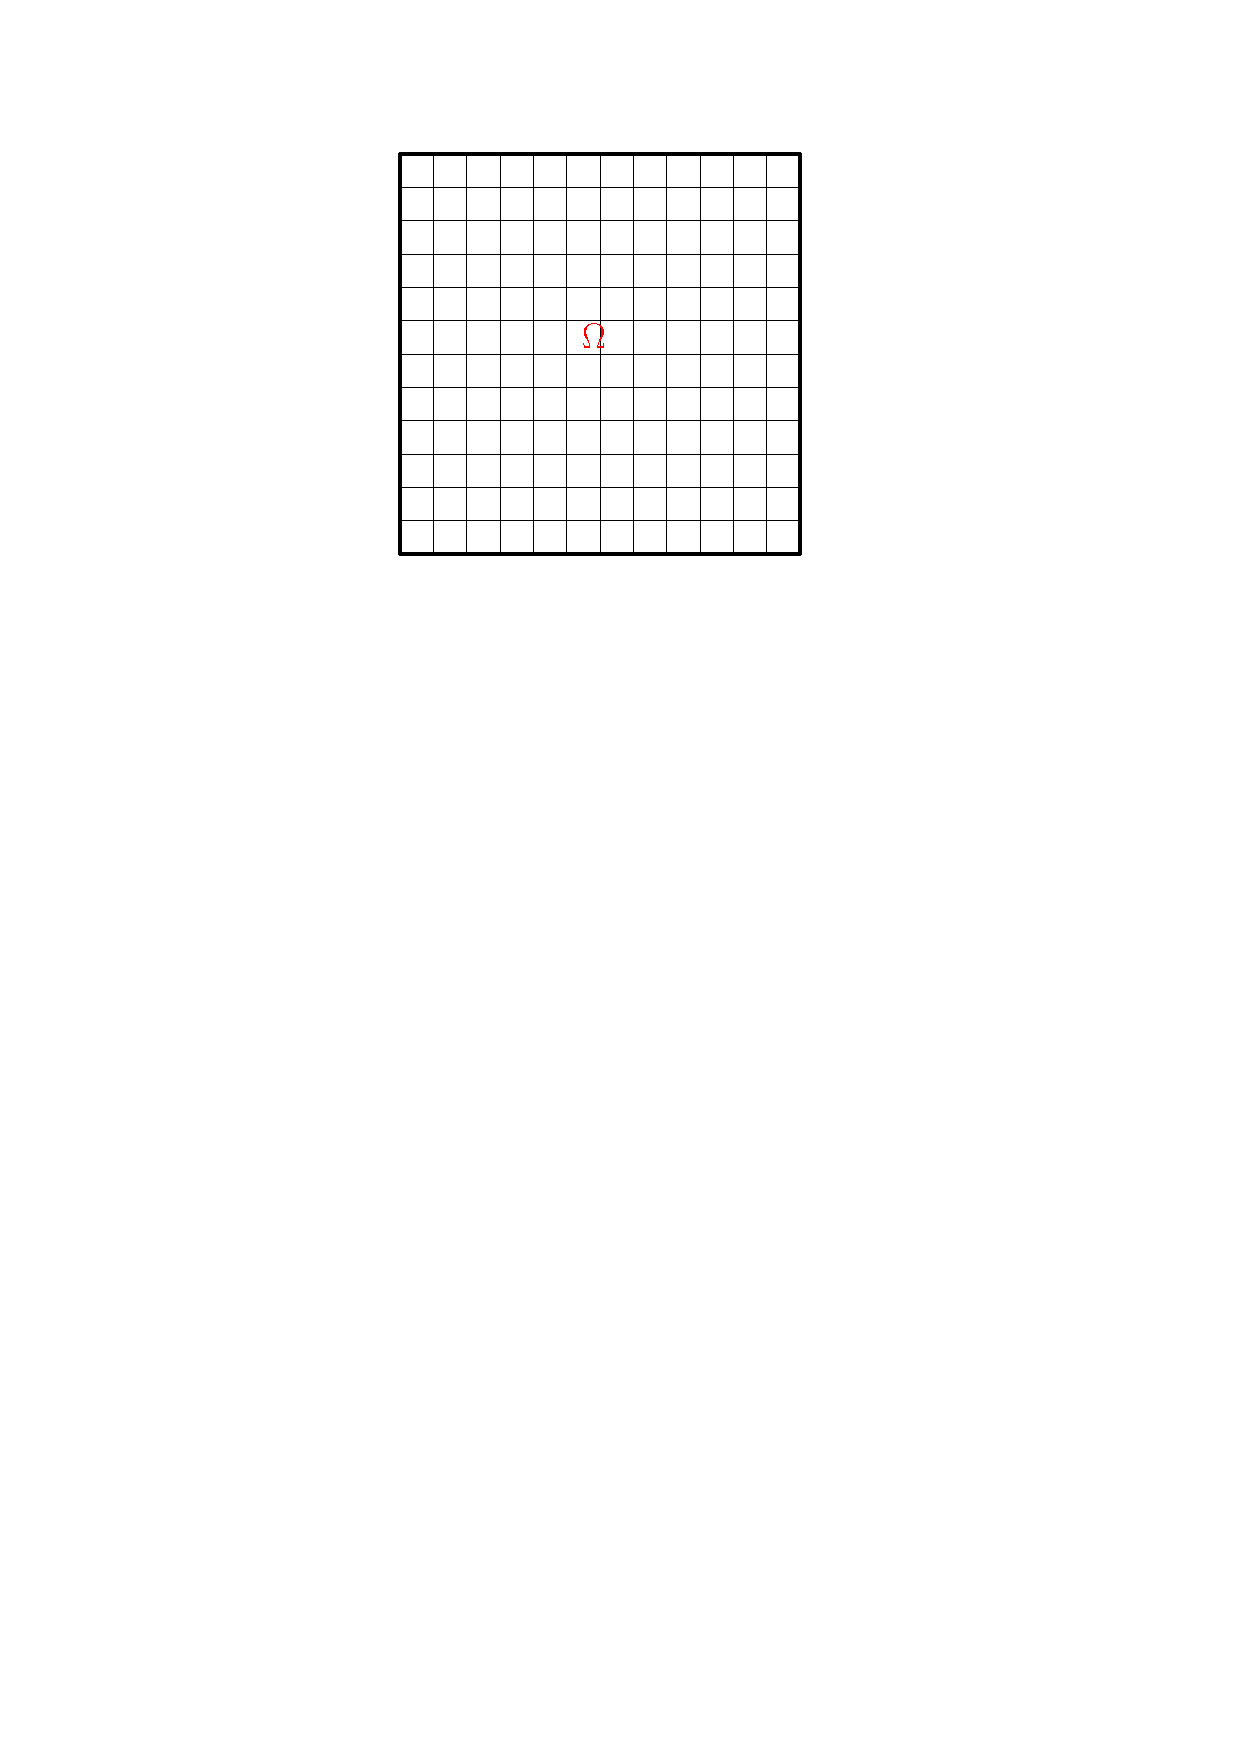
\includegraphics[width=0.5\textwidth]{./pics/domain.pdf}
	\end{tabular}
	\caption{\footnotesize The total computational domain.}\label{fig3: domain}
\end{figure}

\begin{enumerate}
	\item	Compute Schur complement matrix $ S $.
	\item	Further divide the unknowns of the interface into primal and dual subspaces and construct the preconditioner $ S_{BDDC} $ in a parallel fashion.
	\item	Solve the linear system for interface unknowns by using preconditioned conjugate gradient solver.
	\item Calculate the interior unknown through a recovery process.
\end{enumerate}


\begin{figure}[h]
	\centering
	\begin{tabular}{c}
		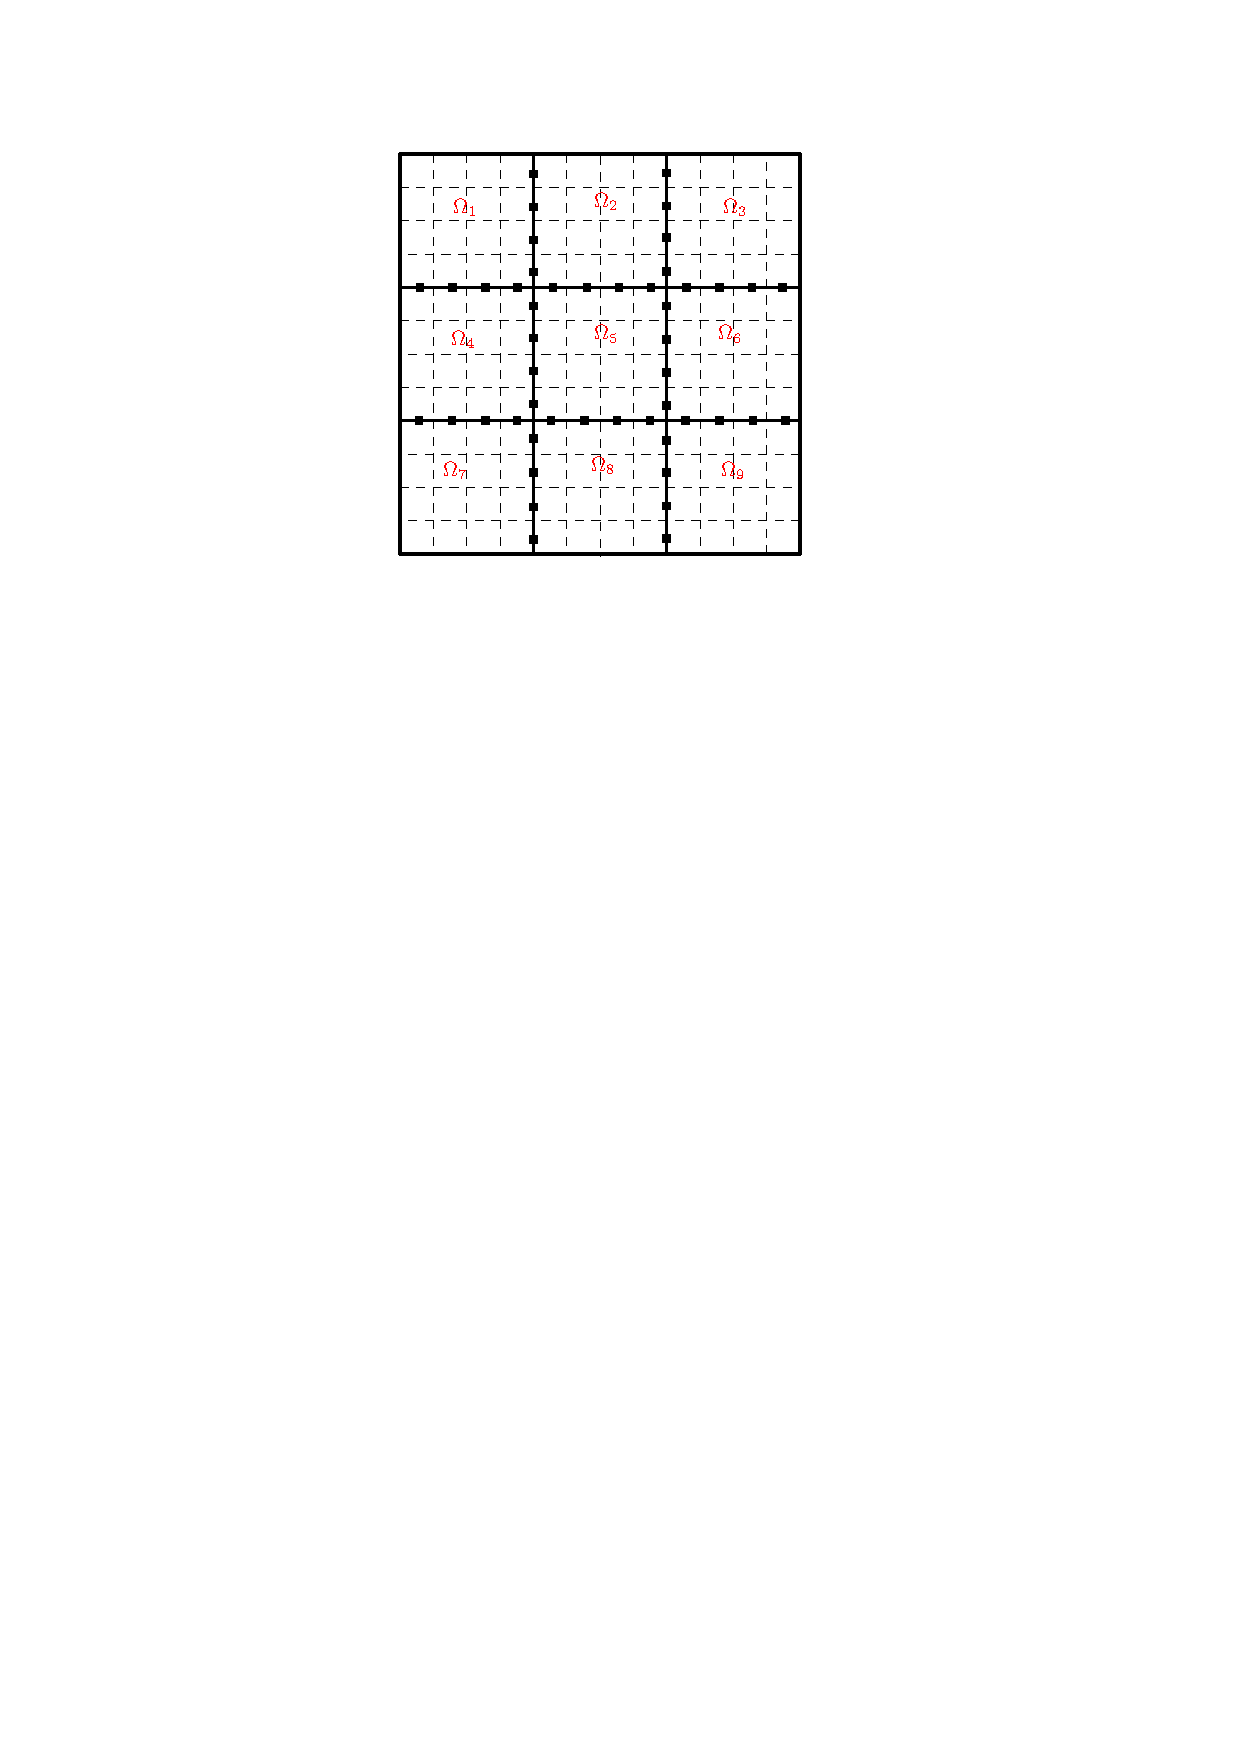
\includegraphics[width=0.6\textwidth]{./pics/domain2.pdf}
	\end{tabular}
	\caption{\footnotesize Decomposed computational .}\label{fig4: domain1}
\end{figure}


\subsection{Schur complement}
%\begin{figure}[H]
%	\centering
%	\begin{tabular}{c}
%		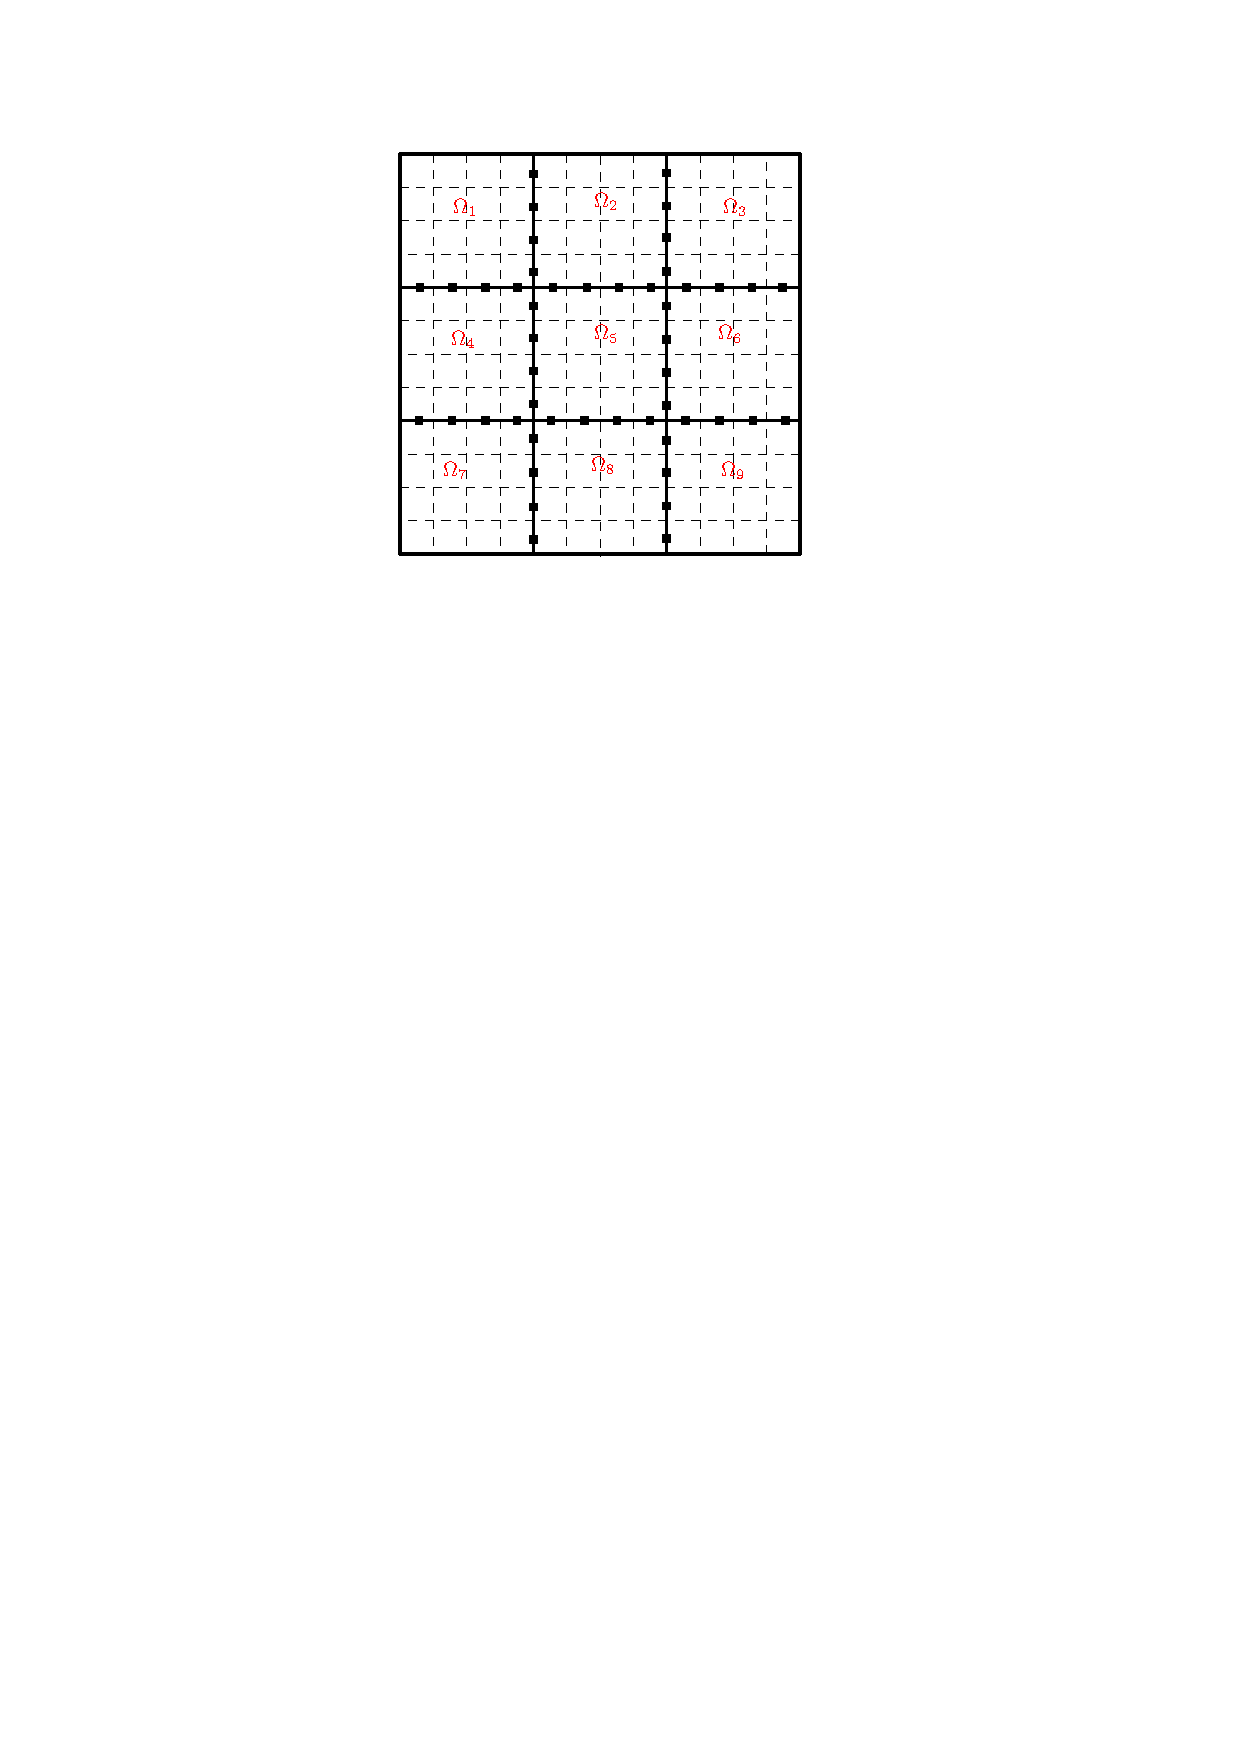
\includegraphics[width=0.35\textwidth]{./pics/domain2.pdf}
%	\end{tabular}
%	\caption{\footnotesize Decomposed computational domain after implementation of Schur Complement method containing interior and interface quantities.}\label{fig4: BDDC2}
%\end{figure}

In Fig. 4.4 , the solid squares contain the unknown variables on the interface between each subdomain. These variables are on the boundary edge which is shared by adjacent elements on corresponding subdomains and should be calculated in the global matrix through Schur complement. The calculation process is given in Eq. \eqref{eq:schur}. The goal of this step is to distribute the multiple square sub-matrices onto each processor for computing the inverse matrix locally. In doing so, the size of the global matrix decreases and includes information from the interface only. 

Denote the weak Galerkin solution on each subdomain $ \Omega_{j} $.  For the consistency with Eq. (1), we use $ \mathbf{u}_{h} $  to represent the weak Galerkin solution on each $ \Omega_{j} $. To define the Schur complement system, the DOFs on every subdomain are partitioned by interior and interface categories. The unknown function becomes $ \mathbf{u}_{h} = [\mathbf{u}_{I0}, \mathbf{u}_{Ib}, \mathbf{u}_{\Gamma b}] $, $ \mathbf{v}_{h} = [\mathbf{v}_{I0}, \mathbf{v}_{Ib}, \mathbf{v}_{\Gamma b}] $ and denote the interior unknown variable $ \mathbf{u}_{i} = [\mathbf{u}_{I0}, \mathbf{u}_{Ib}] $ on the interface we have $ \mathbf{u}_{\Gamma} = \mathbf{u}_{\Gamma b} $ . The same rule applies to the other known variable $ \mathbf{v}_I = [\mathbf{v}_{I0}, \mathbf{v}_{Ib}] $ , $ \mathbf{v}_{\Gamma} = \mathbf{v}_{\Gamma b} $ . 

The governing equation in matrix form can be written as 

\begin{equation}
\begin{pmatrix}
A_{II}^{u} & (A_{\Gamma I}^{u})^{T} & 0 & 0 \\
A_{\Gamma I}^{u} & A_{\Gamma \Gamma}^{u} & 0 & A_{\Gamma \Gamma}^{uv} \\
0 & 0 & A_{II}^{v} & (A_{\Gamma I}^{v})^{T} \\
0 & A_{\Gamma \Gamma}^{uv} & A_{\Gamma I}^{v} & A_{\Gamma \Gamma}^{v} 
\end{pmatrix} 
\begin{pmatrix}
\mathbf{u}_{I} \\ \mathbf{u}_{\Gamma} \\ \mathbf{v}_{I} \\ \mathbf{v}_{\Gamma}
\end{pmatrix} = \begin{pmatrix}
\mathbf{f}_{I}^{u} \\ \mathbf{f}_{\Gamma}^{u} \\ \mathbf{f}_{i}^{v} \\ \mathbf{f}_{\Gamma}^{v} 
\end{pmatrix}
\end{equation}
%
%We apply Schur complement method to convert the interior unknowns which give the following equations

The interface stiffness matrix has the form as following
\begin{equation}
S_{\Gamma \Gamma}^{(j)} = A_{\Gamma \Gamma}^{(j)} - 
\begin{bmatrix}
A_{\Gamma I}^{(j)}
\end{bmatrix} 
\begin{bmatrix}
A_{II}^{(j)}
\end{bmatrix}^{-1}
\begin{bmatrix}
A_{\Gamma I}^{(j)}
\end{bmatrix}^{T}.
\end{equation}

%The loading force along the interface has the form
%\begin{equation}
%f_{\Gamma}^{(j)} = b_{\Gamma}^{(j)} - 
%\begin{bmatrix}
%A_{\Gamma I}^{(j)} 
%\end{bmatrix} 
%\begin{bmatrix}
%A_{II}^{(j)}
%\end{bmatrix}^{-1} 
%b_{I}^{(j)}
%\end{equation}

The assembled matrix form is then
\begin{equation}
S_{\Gamma \Gamma} = \sum_{j = 1}^{N} {R_{\Gamma}^{(j)}}^{T} S_{\Gamma \Gamma}^{(j)}R_{\Gamma}^{(j)} ,
\end{equation}
where $ R_{\Gamma}^{j} $ is the mapping vector to convert unknown variables between the global interface $ \Gamma $ and the local interface $ \Gamma_i $ on subdomains $ \Omega_j $

Therefore, the global interface problem is constructed as 
\begin{equation}
S_{\Gamma \Gamma } \begin{pmatrix}
\mathbf{u}_{\Gamma} \\ \mathbf{v}_{\Gamma}
\end{pmatrix} = 
\begin{pmatrix}
\mathbf{f}_{\Gamma}^{u} \\ \mathbf{f}_{\Gamma}^{v}
\end{pmatrix}
\end{equation}

After the Schur complement, the global matrix size decreases containing information from the interface only. Even though the number of DOFs in the global matrix $ S_{\Gamma} $ is drastically decreased, the size of the global matrix and amount of parallel computing overhead is still too large. The computational space and time limitations remain a bottleneck that prevent us from demonstrating the effectiveness and efficiency of the method. Therefore, we introduce the preconditioner to accelerate performance. To obtain the preconditioner within the parallel framework, we divide the interface problem into primal and dual subspaces, the details of which are provided in the following section.

\subsection{Primal and dual spaces}

\begin{figure}[h]
	\centering
	\begin{tabular}{c}
		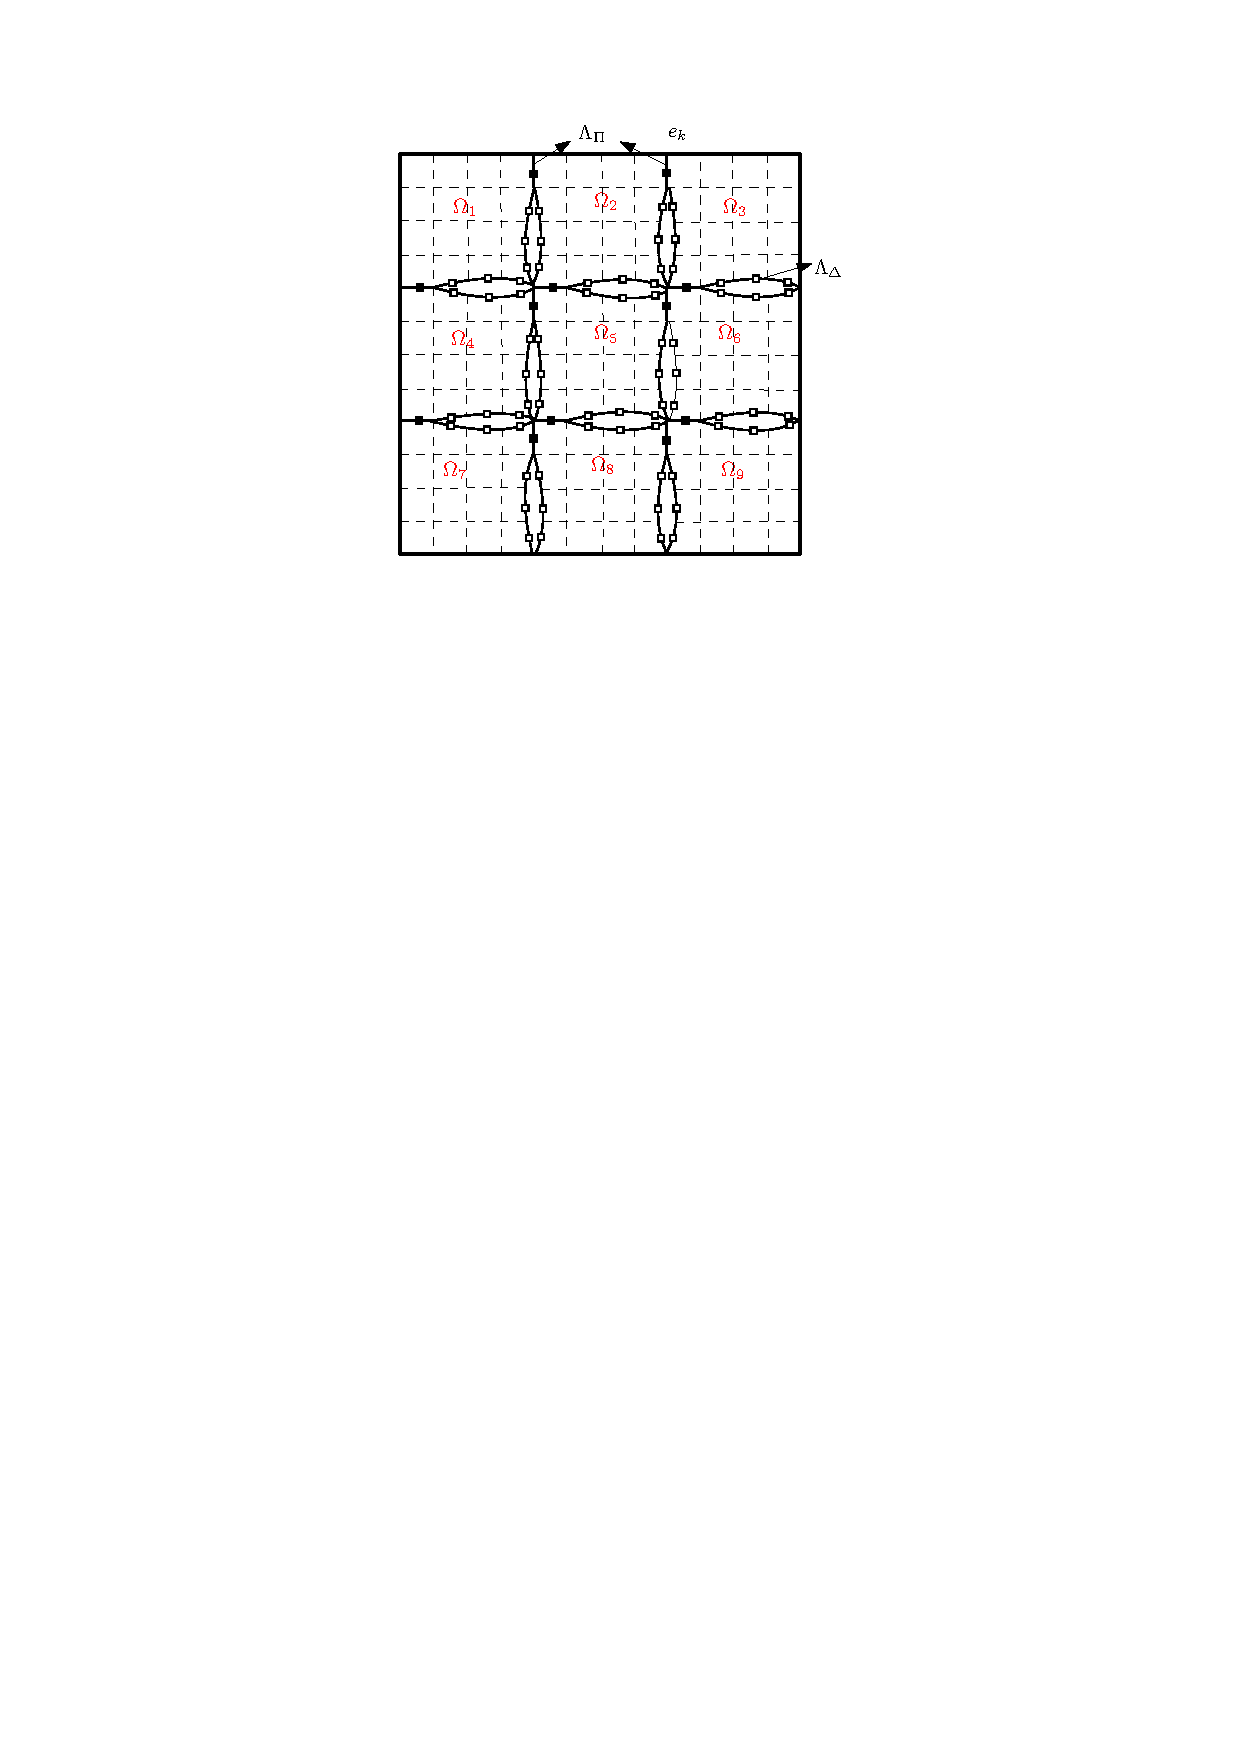
\includegraphics[width=0.6\textwidth]{./pics/domain3.pdf}
	\end{tabular}
	\caption{\footnotesize BDDC computational domain with only one cell boundary.}\label{fig5: BDDC3}
\end{figure}

In Fig. \ref{fig5: BDDC3}, we split the interface into two spaces - primal and dual. The primal space consists of the solid squares, which are the constraints between each subdomain. These are the only unknown variables globally. The dual spae consists of the hollow squares which represent the unknown variables local to each subspace.  We connect the information from hollow squares in  dual space to those in primal space through the preconditioner. The remaining solid squares are unknown variables in primal space. They are the only degrees of freedom which are communicated and calculated through MPI functions.  

One important feature of the BDDC method is the boundedness of the condition number when the number of subdomains increases due to an appropriate choice of preconditioner. The condition number grows very slowly with increasing number of elements in each subdomain. In other words, the total number of iterations within the linear solver is also bounded. This helps the method scale well with the number of subdomains and problem size. 

In the BDDC formulation, primal constraints are introduced over edges/faces. To define the preconditioner for the Schur complement problem, the interface space $ \Lambda_{\Gamma}^{(j)} $ is a partitioned into two spaces, dual, $ \Lambda_{\Delta}^{(j)} $  and primal, $ \Lambda_{\Pi}^{(j)} $. The dual space, $ \Lambda_{\Delta}^{(j)} $, corresponds to the subset of function in $ \Lambda_{\Gamma}^{(j)} $.

We define the partially assembled space as:
\begin{equation} \label{eq:dp}
\hat{\Lambda}_{\Gamma} = \hat{\Lambda}_{\Pi} \oplus (\sum_{i = 1}^{N} \Lambda_{\Delta}^{(j)})
\end{equation}
where $ \hat{\Lambda}_{\Pi} $ is the assembled global primal space, single valued on $ \Gamma $, which is formed by assembling the local primal space, $ \Gamma_{\Pi}^{(j)} $. The BDDC preconditioner has been viewed as solving a finite element problem on partially assembled finite element space, $ \hat{\Lambda}_{\Pi} $, to precondition the Schur complement problem whose solution lies in the fully assembled space $ \hat{\Lambda}_{\Gamma} $.

The key components of the BDDC preconditioner \cite{eisenstat1981efficient} are the following:
\begin{itemize}
	\item 	An averaging operator which restricts functions from $ \Lambda_{\Gamma} $  to $ \hat{\Lambda}_{\Gamma} $
	\item	A positive scaling factor $ \delta_{i}^{\dagger} (e_k) $ is defined for each interface $ e_k $ of the subdomain $ \Omega_j $ such that $ \delta_{i}^{\dagger} (e_k) + \delta_{j}^{\dagger}(e_{k}) = 1 $ where $ e_k = \partial \Omega_i \cap \partial \Omega_j$
	\item	Define $ D_{\Gamma}^{(i)} $ as the diagonal matrix formed by setting the diagonal entries corresponding to each nodal degree of freedom on $ e_k $ to $ \delta_{i}^{\dagger} (e_k) $
	\item	Define $ R_{D, \Gamma} : \hat{\Lambda}_{\Gamma} \rightarrow \Lambda_\Gamma$ as the product of $ R_{D, \Gamma} := D_{\Gamma} R_{\Gamma} $
\end{itemize}


We interpret the Eq. \eqref{eq:governMatrix} by using the unknown variable function $ \mathbf{u}_{\Gamma} = [\mathbf{u}_{r}, \mathbf{u}_{c}]^{T} $. The matrix can be written as
\begin{equation}\label{eq:globalMatrix}
\begin{pmatrix}
A_{rr}^{(1)} & 0 & 0 & \cdots & 0 & A_{rc}^{(1)}\\
0 & A_{rr}^{(2)} & 0 & \cdots & 0 & A_{rc}^{(2)} \\
0 & 0 & A_{rr}^{(3)} & \cdots & 0 & A_{rc}^{(3)} \\
\vdots & \vdots & \vdots & \ddots & \vdots & \vdots \\
0 & 0 & 0 & \cdots & A_{rr}^{(N)} & A_{rc}^{(N)}\\
A_{cr}^{(1)} & A_{cr}^{(2)} & A_{cr}^{(3)} & \cdots & {A_{cr}^{(N)}} & A_{cc} \\
\end{pmatrix} 
\begin{pmatrix}
\underline{\mathbf{u}}_{r}^{(1)} \\ \underline{\mathbf{u}}_{r}^{(2)}  \\ \underline{\mathbf{u}}_{r}^{(3)} \\ \vdots \\ \underline{\mathbf{u}}_{r}^{(N)}  \\ \underline{\mathbf{u}}_{\Pi}
\end{pmatrix} =
\begin{pmatrix}
f_{r}^{(1)} \\ f_{r}^{(2)}  \\ f_{r}^{(3)} \\ \vdots \\ f_{r}^{(N)}  \\ f_{\Pi}
\end{pmatrix}
\end{equation}
where the subscript $ c $ represents the unknown variables of black square constraints and the subscript $ r $ denotes the remaining unknown variable. For example, on subdomain $ (j) $, $ \mathbf{u}_{r}^{(j)} = \mathbf{u}_{I}^{(j)} \cup \mathbf{u}_{\Delta}^{(j)} $.

From the interface unknowns in the primal spaces, in Eq. \eqref{eq:dp}, we assemble all primal unknowns together and formulate a global constraints matrix
\begin{equation}
A_{cc} = \sum_{i=1}^{N} A_{\Pi \Pi}^{(j)}
\end{equation}
where $ c $ represents the corner constraints located in only primal space. 

Similar to Eq. \eqref{eq:schur1}, the rest unknown variables matrix can be written in
\begin{equation}
A_{rr}^{(j)} = \begin{bmatrix}
A_{II}^{(j)} & A_{I \Delta}^{(j)} \\
A_{\Delta I}^{(j)} & A_{\Delta \Delta}^{(j)}\\
\end{bmatrix}
\end{equation}

The implementation of the WG-BDDC algorithm is presented in the following manner:
\begin{equation} \label{eq:bddc}
S_{\Gamma_{BDDC}}^{-1}=\hat{R}_{D,\Gamma}^{T} \{ R_{\Gamma, \Delta}^{T} (\sum_{j = 1}^{N}\begin{bmatrix}
0 & {R_{\Delta}^{(j)}}^{T}
\end{bmatrix} \begin{bmatrix}
A_{II}^{(j)} & A_{I \Delta}^{(j)} \\
A_{\Delta I}^{(j)} & A_{\Delta \Delta}^{(j)}
\end{bmatrix}^{-1} \begin{bmatrix}
0 \\ R_{\Delta}^{(j)}\\
\end{bmatrix} )  R_{\Gamma \Delta} + \Phi S_{\Pi}^{-1} \Phi^{T}\} \hat{R}_{D, \Gamma}
\end{equation}
Similar to block Cholesky method in Eq. \eqref{eq:schur}, the preconditioner is assembled by local inverse and global inverse where the matrix $ \Phi $ represents the connection between Schur complement $ S $ and global stiffness matrix. In Eq. (40), the main difference is that we assemble the global matrix from multiple non-overlapped subdomains and the mapping matrix $ \hat{R} $ is applied on each subdomain.

The matrix $ \Phi $ is computed using
\begin{equation} \label{eq:bddc1}
\Phi = R_{\Gamma\Pi}^{T} - R_{\Gamma \Delta}^{T} \sum_{j = 1}^{N} \begin{bmatrix}
0 & {R_{\Delta}^{(j)}}^{T} 
\end{bmatrix} \begin{bmatrix}
A_{II}^{(j)} & A_{I \Delta}^{(j)} \\
A_{\Delta I}^{(j)} & A_{\Delta \Delta}^{(j)}
\end{bmatrix}^{-1} \begin{bmatrix}
{A_{\Pi I}^{(j)}}^{T} \\ {A_{\Pi \Delta}^{(j)}}^{T} 
\end{bmatrix} R_{\Pi}^{(j)} ,
\end{equation}

The matrix $ S_{\Pi} $ is the global coarse system matrix computed by
\begin{equation}\label{eq:bddc2}
S_{\Pi} = \sum_{j = 1}^{N} {R_{\Pi}^{(j)}}^{T} \{ A_{\Pi \Pi}^{(j)} - \begin{bmatrix}
A_{\Pi I}^{(j)} & A_{\Pi \Delta}^{(j)}
\end{bmatrix}  \begin{bmatrix}
A_{II}^{(j)} & A_{I\Delta}^{(j)} \\
A_{\Delta I}^{(j)} & A_{\Delta \Delta}^{(j)}
\end{bmatrix}^{-1} \begin{bmatrix}
{A_{\Pi I}^{(j)}}^{T} & {A_{\Pi \Delta}^{(j)}}^{T}
\end{bmatrix} \} R_{\Pi}^{(j)} .
\end{equation}
The major computational cost of calculating the global preconditioner lies in the inversion of the local matrix $ \begin{bmatrix}
A_{II}^{(j)} & A_{I\Delta}^{(j)} \\
A_{\Delta I}^{(j)} & A_{\Delta \Delta}^{(j)}
\end{bmatrix}^{-1}  $, and which is distributed and calculated on each processor $ (j) $. Thus the synchronization overhead is reduced to a very low level.

The BDDC preconditioner has the following form
\begin{equation}
S_{\Gamma_{BDDC}}^{-1} = R_{D, \Gamma}^{T} \tilde{S}_{\Gamma\Gamma}^{-1} R_{D, \Gamma}.
\end{equation}

The global interface problem after preconditioning can be written as
\begin{equation}
S_{\Gamma_{BDDC}}^{-1} S_{\Gamma \Gamma} \mathbf{u}_{\Gamma} = S_{\Gamma_{BDDC}}^{-1} \mathbf{f}_{\Gamma}.
\end{equation}

The preconditioned conjugate gradient is applied to solve the above linear system in Eq. (44). Theoretically, the condition number should be bounded, where
\begin{equation}
\kappa (S_{\Gamma_{BDDC}}^{-1} \hat{S}_{\Gamma \Gamma}) \leq C (1 + log (\frac{kH}{h}))^{2}
\end{equation}
for a second order elliptic problem. The constant $ C $  is independent of solution order $ p $, element size $ h $,  and subdomain size $ H $ . Thus, the condition number and the number of iterations to achieve convergence are independent of the number of subdomains and only depend upon the accuracy order and subdomain size.  

\subsection{Preconditioned Conjugate Gradient Method}
The preconditioned conjugate gradient (PCG) method is adopted as the linear solver for BDDC method. The construction of preconditioner is crucial for PCG method. The BDDC preconditioner combines the solution of the local problem on each subdomain with the solution of a global coarse problem while treating the coarse degrees of freedoms as unknowns. 


The conjugate gradient (CG) method is an effective iterative numerical method for solving large-scale symmetric and positive definite linear systems. The method is straightforward to implement and has the capability to handle complex domains and boundary conditions. 

The preconditioned conjugate gradient method has been reported by Bramble and Pasciak \cite{bramble1988preconditioning} to iteratively solve the symmetric saddle point problems. It inherits beneficial features of CG  and extends it to a better performance. This method is applied to a sparse system which is too large to handle by a direct method such as the Cholesky decomposition.

The details of the PCG method are summarized by Algorithm I. The major effort in preconditioning is to assemble the global preconditioner matrix. Then, the CG method is applied to solve the preconditioned global matrix. By doing this, we can obtain the global interface solution with minimal iterations. Both global and local matrices are large and sparse, and we directly take advantage of the open source library LAPACK/BLAS \cite{anderson1999lapack}.

The algorithm of PCG method is following:

\begin{algorithm}[H] \label{al:pcg}
	\SetKwInOut{Input}{Input}
	\SetKwInOut{Output}{Output}
	
	% \underline{function Euclid} $(a,b)$\;
	\Input{$r_0:=b-M\underline{\mathbf{u}}_0$\\
		$z_0:=S^{-1}_{\Gamma_{BDDC}}r_0$\\
		$p_0:=z_0$\\
		$k\ :=0$}
	%\Output{$\gcd(a,b)$}
	\underline{Repeat} \;%$(a,b)$\;
	\begin{flalign*}
	\vspace{-20pt}
	\alpha_k:&=\frac{r_k^Tz_k}{p_k^TAp_k}&\\
	\underline{U}_{k+1}:&=\underline{\mathbf{u}}_k+\alpha_kp_k\\
	r_{k+1}:&=r_k-\alpha_kAp_k
	\end{flalign*}
	\eIf{$r_k$ is sufficiently small}
	{
		return $\mathbf{u}_{k+1}$\;
	}
	{
		\begin{flalign*}
		z_{k+1}:&=S^{-1}_{\Gamma_{BDDC}}r_{k+1}&\\
		\beta_k:&=\frac{z_{k+1}^T r_{k+1} }{z_k^T r_k}\\
		p_{k+1}:&=z_{k+1}+\beta_kp_k\\
		k:&=k+1
		\end{flalign*}
	}
	\caption{Preconditioned Conjugate Gradient Algorithm}
\end{algorithm}
where $ r $ is the residue vector, $ p $ is the orthogonal direction vector and $ k $ is the iteration number. 


The Lanczos\cite{cullum2002lanczos} matrix is applied to estimate the upper and lower eigenvalue bounds. The matrix is in a tridiagonal form and generated from the PCG iterations.
The global preconditioner matrix $ S^{-1}_{\Gamma_{BDDC}} $ is converted into a tridiagonal matrix $ L_{mm} $. When the $ m $ equals to the dimension of $ M $, $ L_{mm} $ is similar to $ S^{-1}_{\Gamma_{BDDC}} $. Then we calculate the eigenvalues of $ L_{mm} $ and obtain the condition number from calculating the ratio of  the maximum and minimum eigenvalues.



\subsection{Recover local information}

The solution on the interface, $ \mathbf{u}_{\Gamma} $ , is obtained iteratively from the PCG solver. The small global vector result is communicated and shared by all processors. For each processor, the local interior DOFs, $ \mathbf{u}_{I} $, can be recovered through the following equations. The local DOFs of interior unknowns and interface unknowns have the following relation

\begin{equation}
A_{II}^{u^{(j)}} \mathbf{u}_{I}^{(j)} + (A_{\Gamma I}^{u^{(j)}})^{T} \mathbf{u}_{\Gamma}^{(j)} = f_{I}^{(j)}
\end{equation}

Since $ u_{\Gamma}^{(j)} $ has been obtained from the PCG linear solver and $ f_{I}^{(j)} $ is known, the local recovery is obtained by
\begin{equation} \label{eq:recover}
\mathbf{u}_{I}^{(j)} =  (A_{II}^{u^{(j)}})^{-1} (f_{I}^{(j)} - (A_{\Gamma I}^{u^{(j)}})^{T} \mathbf{u}_{\Gamma}^{(j)})
\end{equation} 
where each local processor inverts the local positive definite square matrix $ A_{II}^{u^{(j)}} $. The compute time for $  (A_{II}^{u^{(j)}})^{-1} $ decreases significantly as we increase the number of subdomains. 


\subsection{Workflow of the parallel computing scheme}

Message Passing Interface (MPI) \cite{gropp1996high} is portable and widely used as the communicator. We applied MPI to exchange the information between each non-overlapping subdomain. MPI provides a standard set of Fortran subprogram definitions. Intel MKL supports the modern MPI version which allows us to migrate the software on a variety of platforms. Besides, the MPI subprograms introduce the minimum overhead in both coding and testing stages.

The workflow of parallel computing scheme is following:
\begin{figure}[ht]
	\centering
	\begin{tabular}{c}
		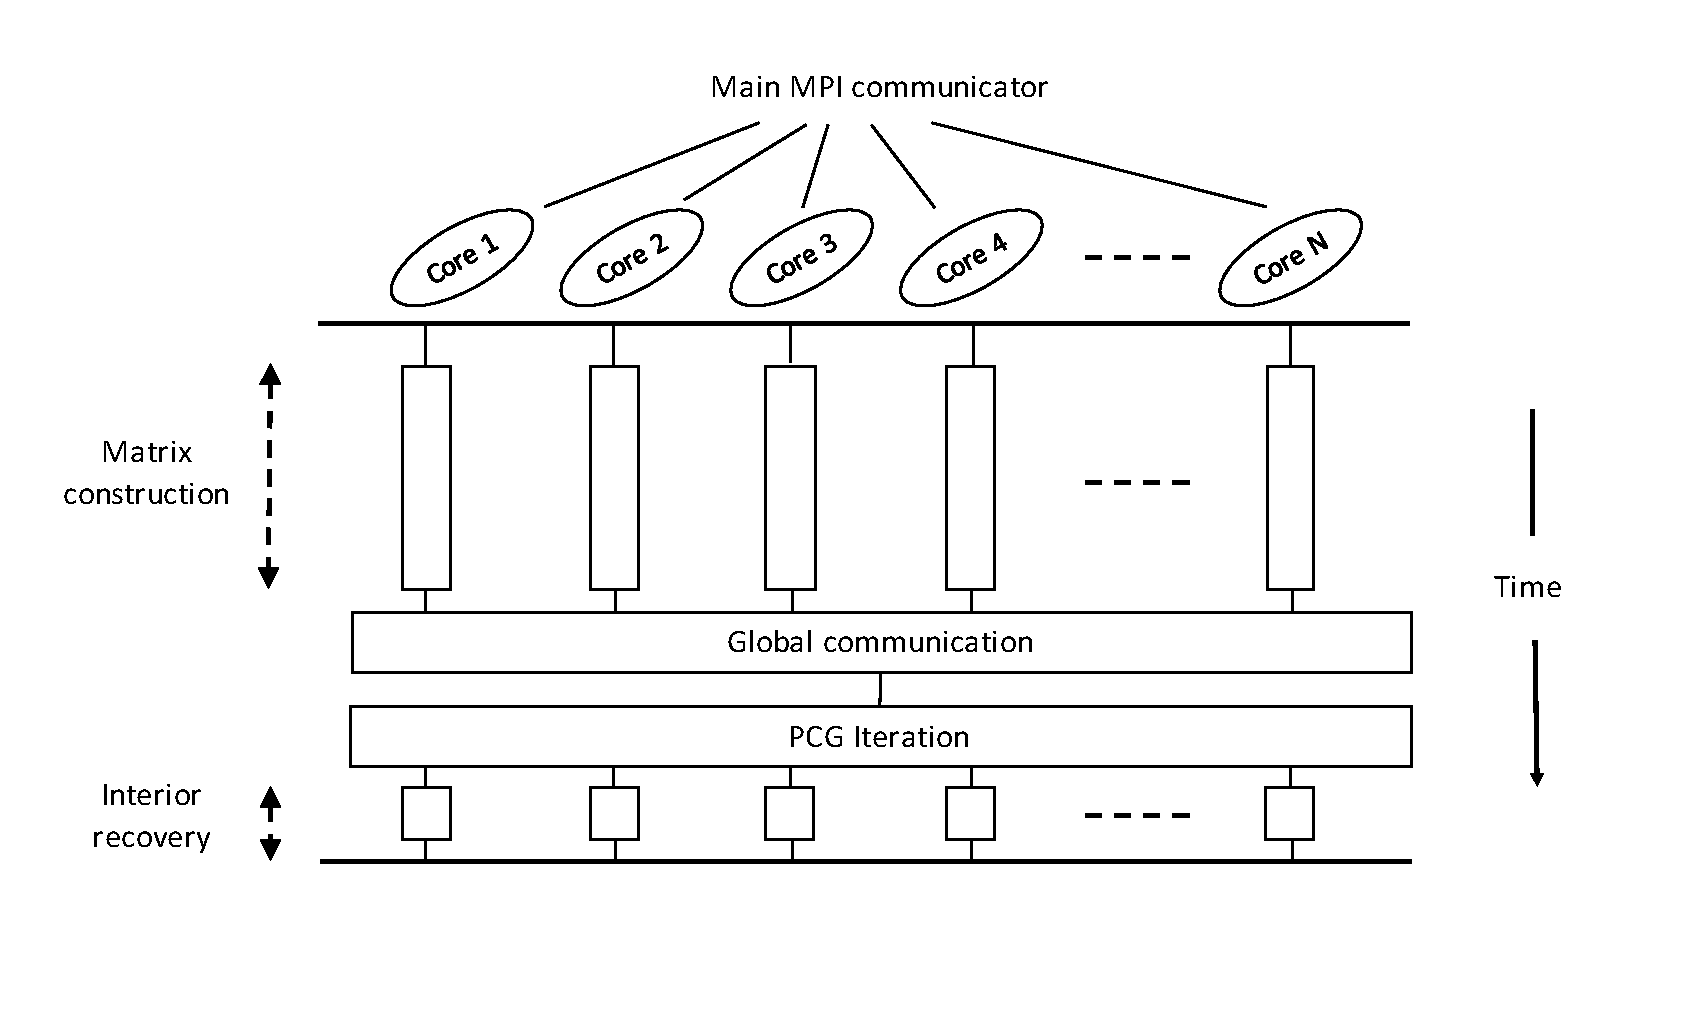
\includegraphics[width=0.8\textwidth]{./pics/mpi_flow.eps}
	\end{tabular}
	\caption{\footnotesize Parallel computing work flow.}\label{fig6: mpi}
\end{figure}
\begin{enumerate}
	\item	MPI communicator initiates work and distributes the parameters, configuration and mesh data to all the processors in the same time. The global matrix $ M $ is divided into two spaces primal and dual. For each processor, it reads the corresponding geometry and connectivity information. 
	\item	For each processor, the local elemental matrices are constructed individually, in Fig. \ref{fig6: mpi} the matrix construction section. The primal matrix $ S_{\Pi} $ is constructed in this step. Every processor deals with one non-overlapping subdomain refers to Eqs. \eqref{eq:bddc1} and \eqref{eq:bddc2}. The local inverse is calculated by using block Cholesky elimination and communicate through interface with global mapping vectors $ R_{D, \Gamma} $.
	\item	Through MPI subprograms, the local matrices are communicated and the global preconditioner is constructed and assembled through each processor. The preconditioner $ S_{\Gamma_{BDDC}}^{-1} $ refers to Eq. \eqref{eq:bddc} which is the assemblage from each individual processor.
	\item	The global problem, is calculated on every processor with PCG linear solver. The details of PCG solver illustrated in Algorithm \ref{al:pcg}.
	\item	The global solution is reduced to each processor for the local solution recovery, in Fig. \ref{fig6: mpi} interior recovery section. When the global solution in primal space shared with each processors, the local unknown DOFs can be recovered individually by Eq. \eqref{eq:recover}
\end{enumerate}

Throughout this paper, the results from our WG-BDDC code has been obtained on Colonial One, a supercomputing facility at the George Washington University. ColonialOne has total 200+ nodes of Xeon E5-2650 8-core processors. Each processor has 2.6GHz processing speed.



%===============================================
\section{Numerical Results}

\subsection{Poisson Equation}
We can choose different order of basis functions in a WG element for the weak gradient equation among gradient, interior and boundary basis functions. We test different combination orders of interior, boundary and weak gradient shape functions. 

In the first test, we consider the Poisson equation $ -\nabla \cdot (\nabla \mathbf{u}) = \mathbf{f} $. Let $ \Omega = (0, 1) \times (0, 1) $, $ a = I $, and $ \mathbf{f} $ are chosen such that the exact solution is $ u = sin(\pi x) sin(\pi y) $

We choose different weak Galerkin elements for validating our WG-BDDC numerical scheme. The unit square is first decomposed into $ N \times N $ subdomains as the coarse mesh with length $ H = 1 / N $. In every subdomain, all elements are further triangulated into $ 2 n \times n $ triangles, and the finite mesh has the size $ h = 1/(N\times n) $. The preconditioned system is solved by the PCG solver. In every iteration, the $ L^2- $norm of the residual is reduced by a factor of $ 10^{-7} $.

%\begin{table}[H]
%	\setlength{\tabcolsep}{2pt} {
%		\caption{ Performance with $P_{k}P_{k-1}P_{k-1}^2$.}
%		\label{Tab:case1_PkPk-1Pk-1}
%		\vspace{-5pt}
%		\begin{center}
%		%	\scalebox{0.6}{
%				\begin{tabular}{c|cccc|c|cccc}
%					\hline
%					\multirow{2}{*}{\#sub} &\multicolumn{4}{c|}{$k=1$ and $H/h=8$} &\multirow{2}{*}{$H/h$} &\multicolumn{4}{c}{$k=1$ and \#sub=64}\\ 
%					& Cond.   & Iter. &$L^2$-error & $ O $ & & Cond.   & Iter. &$L^2$-error &$ O $ \\
%					\hline
%					$4\times 4$     &2.217 &5 &1.6013e-3 &- &4   &1.722 &7   &1.6013e-3 & -\\
%					$8\times 8$     &2.390 &9 &3.9939e-4 & 2.0 &8   &2.390 &9   &3.9939e-4& 2.0\\
%					$16\times 16$ &2.335 &8 &9.9789e-5 & 2.0 &16 &3.245 &10 &9.9789e-5 & 2.0\\
%					$32\times 32$ &2.325 &8 &2.4944e-5 & 2.0 &32 &4.239 &11 &2.4944e-5 & 2.0 \\
%					\hline
%					\multirow{2}{*}{\#sub} &\multicolumn{4}{c|}{$k=2$ and $H/h=8$} &\multirow{2}{*}{$H/h$} &\multicolumn{4}{c}{$k=2$ and \#sub=64}\\ 
%					& Cond.   & Iter. &$L^2$-error & $ O $ & & Cond.   & Iter. &$L^2$-error & $ O $  \\
%					\hline
%					$4\times 4$    &3.528 & 8  &7.1456e-5 & -  &4   &2.900 &10 &7.1456e-5 & - \\
%					$8\times 8$    &3.803 &10 &8.9214e-6 & 3.0 &8   &3.803 &10 &8.9214e-6 & 3.0 \\
%					$16\times 16$&3.768 &10 &1.1150e-6 & 3.0 &16 &4.957 &12 &1.1150e-6 & 3.0 \\
%					$32\times 32$&3.758 &10 &1.3938e-7 & 3.0 &32 &6.218 &13 &1.3938e-7 & 3.0\\
%					\hline
%				\end{tabular}
%		%	}
%		\end{center} }
%	\end{table}

\vspace{5mm}
\begin{table}[H]
	\setlength{\tabcolsep}{2pt} {
		\vspace{-5pt}
		\begin{center}
			%	\scalebox{0.6}{
			\begin{tabular}{c|cccc|cccc}
				\hline
				\multirow{2}{*}{\#sub} &\multicolumn{4}{c|}{$k=1$} &\multicolumn{4}{c}{$k=2$}\\ 
				& Cond.   & Iter. &$L^2$-error & $ O $ & Cond.   & Iter. &$L^2$-error &$ O $ \\
				\hline
				$4\times 4$     &2.217 &5 &1.6013e-3 &-  &3.528 & 8  &7.1456e-5 & - \\
				$8\times 8$     &2.390 &9 &3.9939e-4 & 2.0 &3.803 &10 &8.9214e-6 & 3.0\\
				$16\times 16$ &2.335 &8 &9.9789e-5 & 2.0 &3.768 &10 &1.1150e-6 & 3.0\\
				$32\times 32$ &2.325 &8 &2.4944e-5 & 2.0 &3.758 &10 &1.3938e-7 & 3.0\\
				\hline
			\end{tabular}
			%	}
		\end{center} }
		\caption{The accuracy and convergence properties of the $P_{k}P_{k-1}P_{k-1}^2$ element on different numbers of subdomains where each subdomain has 128 triangular elements.}
		\label{Tab:case1_PkPk-1Pk-1Row1}
	\end{table}
	
	\vspace{5mm}
	\begin{table}[H]
		\setlength{\tabcolsep}{2pt} {
			\vspace{-5pt}
			\begin{center}
				%	\scalebox{0.6}{
				\begin{tabular}{c|cccc|cccc}
					\hline
					\multirow{2}{*}{$ H/h $} &\multicolumn{4}{c|}{$k=1$}  &\multicolumn{4}{c}{$k=2$}\\ 
					& Cond.   & Iter. &$L^2$-error & $ O $ & Cond.   & Iter. &$L^2$-error &$ O $ \\
					\hline
					4   &1.722 &7   &1.6013e-3 & - &2.900 &10 &7.1456e-5 & - \\
					8   &2.390 &9   &3.9939e-4& 2.0 &3.803 &10 &8.9214e-6 & 3.0\\
					16 &3.245 &10 &9.9789e-5 & 2.0 &4.957 &12 &1.1150e-6 & 3.0\\
					32 &4.239 &11 &2.4944e-5 & 2.0 &6.218 &13 &1.3938e-7 & 3.0\\
					\hline
				\end{tabular}
				%	}
			\end{center} }
			\caption{The accuracy and convergence  $P_{k}P_{k-1}P_{k-1}^2$ scheme on different number of fine element in each subdomain. The entire computational domain is partitioned into 64 non-overlapping subdomains.}
			\label{Tab:case1_PkPk-1Pk-1Row2}
		\end{table}
		
		In above examples, the largest test case contains more than 1 million degree of freedoms. 
		The first test is implemented for weak Galerkin element with $ u_0 \in P_k, u_b \in P_{k - 1} $, and $ \nabla_w u \in P_{k - 1} $. The Tables \ref{Tab:case1_PkPk-1Pk-1Row1} and \ref{Tab:case1_PkPk-1Pk-1Row2} show the condition number of Lanczos matrix and the iteration number in the PCG solver. From the Table \ref{Tab:case1_PkPk-1Pk-1Row1} and Table \ref{Tab:case1_PkPk-1Pk-1Row2}, we can see that the condition number does not increase proportionally with the increasing number of subdomains. It depends upon the resolution of mesh, $ H/h $, as $ (1 + log(\frac{H}{h}))^{2} $. With the increasing number of subdomains, we obtain stable second and third order accuracy results. Similarly, the iteration number is also well-bounded. Due to the fact that the size of global matrix grows at a slower rater than the DOFs in primal space.
		
		
		%	\begin{table}[H] 
		%		\small
		%		\setlength{\tabcolsep}{1pt} {
		%			\caption{ Performance with $P_{k}P_{k}P_{k-1}^2$.}
		%			\label{Tab:case1_PkPkPk-1}
		%			\begin{center}
		%				%\scalebox{0.8}{
		%					\begin{tabular}{c|cccc|c|cccc}
		%						\hline
		%						\multirow{2}{*}{\#sub} &\multicolumn{4}{c|}{$k=1$ and $H/h=8$} &\multirow{2}{*}{$H/h$} &\multicolumn{4}{c}{$k=1$ and \#sub=64}\\ 
		%						& Cond.   & Iter. &$L^2$-error & $O1$ & & Cond.   & Iter. &$L^2$-error & $O$\\
		%						\hline
		%						$4\times 4$ & 2.451 & 7 & 1.0109e-3 & - &$4$ &1.968 &8 &1.0109e-3 &-\\
		%						$8\times 8$ &2.648 &9 &2.5117e-4 &	2.0  &8 &2.648 &9 &2.5117e-4 &2.0 \\
		%						$16\times 16$ &2.629 &9 &	6.2696e-5 &2.0  &16 &3.529 &10 &6.2696e-5 &2.0\\
		%						$32\times 32$ &2.617 &9 &1.5668e-5 &2.0  &32 &4.619 &12 &1.5668e-5 &2.0\\
		%						\hline
		%						\multirow{2}{*}{\#sub} &\multicolumn{4}{c|}{$k=2$ and $H/h=8$} &\multirow{2}{*}{$H/h$} &\multicolumn{4}{c}{$k=2$ and \#sub=64}\\ 
		%						& Cond.   & Iter. &$L^2$-error &  $\lambda_1$ & & Cond.   & Iter. &$L^2$-error & $\lambda_1$\\
		%						\hline
		%						$4\times 4$ & 3.805 &8 &6.6333e-5  &- &4 &3.926 &11 &6.6333e-5  &-\\
		%						$8\times 8$ & 4.003 &12 &8.2709e-6  & 3.0 &8 &4.003 &12 &8.2709e-6  &3.0 \\
		%						$16\times 16$ &3.943 &12 &1.0334e-6  &3.0 &16 &5.084 &13 &1.0334e-6  &3.0\\
		%						$32\times 32$ &3.917 &12 &1.2917e-7  &3.0 &32 &6.329 &13 &1.2918e-7  &3.0\\
		%						\hline
		%					\end{tabular}
		%			%	}
		%			\end{center} }
		%		\end{table}
		
		\vspace{5mm}
		\begin{table}[H]
			%						\small
			\setlength{\tabcolsep}{1pt} {
				\begin{center}
					%\scalebox{0.8}{
					\begin{tabular}{c|cccc|cccc}
						\hline
						\multirow{2}{*}{\#sub} &\multicolumn{4}{c|}{$k=1$} &\multicolumn{4}{c}{$k=2$}\\ 
						& Cond.   & Iter. &$L^2$-error & $O$ & Cond.   & Iter. &$L^2$-error & $O$\\
						\hline
						$4\times 4$ & 2.451 & 7 & 1.0109e-3 & - &3.805 &8 &6.6333e-5  &- \\
						$8\times 8$ &2.648 &9 &2.5117e-4 &	2.0  &4.003 &12 &8.2709e-6  & 3.0 \\
						$16\times 16$ &2.629 &9 &	6.2696e-5 &2.0  &3.943 &12 &1.0334e-6  &3.0\\
						$32\times 32$ &2.617 &9 &1.5668e-5 &2.0  &3.917 &12 &1.2917e-7  &3.0\\
						\hline
					\end{tabular}
					%	}
					\caption{The accuracy and convergence properties of the $P_{k}P_{k}P_{k-1}^2$ element on different numbers of subdomains where each subdomain has 128 triangular elements.}
					\label{Tab:case1_PkPkPk-1 Row1}
				\end{center} }
			\end{table}
			
			\vspace{5mm}
			\begin{table}[H]
				%						\small
				\setlength{\tabcolsep}{1pt} {
					\begin{center}
						%\scalebox{0.8}{
						\begin{tabular}{c|cccc|cccc}
							\hline
							\multirow{2}{*}{$H/h$} &\multicolumn{4}{c|}{$k=1$ and \#sub=64}  &\multicolumn{4}{c}{$k=2$ and \#sub=64}\\ 
							& Cond.   & Iter. &$L^2$-error & $O1$ & Cond.   & Iter. &$L^2$-error & $O$\\
							\hline
							$4$ &1.968 &8 &1.0109e-3 &-&3.926 &11 &6.6333e-5  &-\\
							8 &2.648 &9 &2.5117e-4 &2.0 &4.003 &12 &8.2709e-6  &3.0 \\
							16 &3.529 &10 &6.2696e-5 &2.0  &5.084 &13 &1.0334e-6  &3.0\\
							32 &4.619 &12 &1.5668e-5 &2.0  &6.329 &13 &1.2918e-7  &3.0\\
							\hline
						\end{tabular}
						%	}
					\end{center} }
					\caption{The accuracy and convergence  $P_{k}P_{k}P_{k-1}^2$ scheme on different number of fine element in each subdomain. The entire computational domain is partitioned into 64 non-overlapping subdomains.}
					\label{Tab:case1_PkPkPk-1Row2}
				\end{table}						
				
				
				
				The second test is the weak Galerkin element with order $ u_{0} \in P_{k} $, $ u_{b} \in P_{k} $ and $ \nabla_{w}u \in P_{k - 1} $. In Table \ref{Tab:case1_PkPkPk-1 Row1} and Table \ref{Tab:case1_PkPkPk-1Row2} the condition number has the identical pattern of the theoretical convergence rate. Comparing to the first example, we find that convergence rates and the orders of accuracy have optimal agreement to the degree of polynomial in $ u_{0} $. The maximum number of processors for this example is up 1024. The WG-BDDC method shows optimal scalability.
				
				%\begin{table}[H]
				%	\small
				%	\vspace{-10pt}
				%	\setlength{\tabcolsep}{1pt} {
				%		\caption{Case 1: Performance with $P_{k}P_{k}P_{k}^2$.}
				%		\label{Tab:case1_PkPkPk}
				%		\vspace{-5pt}
				%		\begin{center}
				%			%\scalebox{0.8}{
				%			\begin{tabular}{c|cccc|c|cccc}
				%				\hline
				%				\multirow{2}{*}{\#sub} &\multicolumn{4}{c|}{$k=1$ and $H/h=8$} &\multirow{2}{*}{$H/h$} &\multicolumn{4}{c}{$k=1$ and \#sub=64}\\ 
				%				& Cond.   & Iter. &$L^2$-error & $O$  & & Cond.   & Iter. &$L^2$-error & $O$ \\
				%				\hline
				%				$4\times 4$     &3.671 & 8  &2.1451e-4 &- &4   &3.024 &10 &2.1451e-4 &- \\
				%				$8\times 8$     &3.965 &10 &5.2129e-5 &2.0  &8   &3.965 &10 &5.2129e-5 &2.0 \\
				%				$16\times 16$ &3.934 &10 &1.2937e-5 &2.0  &16 &5.153 &12 &1.2937e-5 &2.0 \\
				%				$32\times 32$ &3.922 &10 &3.2281e-6 &2.0  &32 &6.472 &14 &3.2281e-6 &2.0 \\
				%				\hline	
				%				\multirow{2}{*}{\#sub} &\multicolumn{4}{c|}{$k=2$ and $H/h=8$} &\multirow{2}{*}{$H/h$} &\multicolumn{4}{c}{$k=2$ and \#sub=64}\\ 
				%				& Cond.   & Iter. &$L^2$-error & $O$ & & Cond.   & Iter. &$L^2$-error & $O$ \\
				%				\hline
				%				$4\times 4$     &4.620 &8   &6.7627e-6 &-  & 4  &3.859 &11 &6.7628e-6 &- \\
				%				$8\times 8$     &4.987 &12 &7.8998e-7 &3.0  &8   &4.987 &12 &7.8998e-7 &3.0 \\
				%				$16\times 16$ &4.921 &12 &9.6925e-8 &3.0  &16 &6.235 &13 &9.6931e-8 &3.0 \\
				%				$32\times 32$ &4.901 &12 &1.2058e-8 &3.0  &32 &7.673 &15 &1.2060e-8 &3.0 \\
				%				\hline
				%			\end{tabular}
				%			%}
				%		\end{center} }
				%	\end{table}
				
				\vspace{5mm}
				\begin{table}[H]
					%	\small
					\vspace{-10pt}
					\setlength{\tabcolsep}{1pt} {
						\vspace{-5pt}
						\begin{center}
							%\scalebox{0.8}{
							\begin{tabular}{c|cccc|cccc}
								\hline
								\multirow{2}{*}{\#sub} &\multicolumn{4}{c|}{$k=1$} &\multicolumn{4}{c}{$k=2$}\\ 
								& Cond.   & Iter. &$L^2$-error & $O$  &  Cond.   & Iter. &$L^2$-error & $O$ \\
								\hline
								$4\times 4$     &3.671 & 8  &2.1451e-4 &- &4.620 &8   &6.7627e-6 &- \\
								$8\times 8$     &3.965 &10 &5.2129e-5 &2.0  &4.987 &12 &7.8998e-7 &3.0 \\
								$16\times 16$ &3.934 &10 &1.2937e-5 &2.0  &4.921 &12 &9.6925e-8 &3.0  \\
								$32\times 32$ &3.922 &10 &3.2281e-6 &2.0  &4.901 &12 &1.2058e-8 &3.0\\
								\hline	
							\end{tabular}
							%}
						\end{center} }
						\caption{The accuracy and convergence properties of the $P_{k}P_{k}P_{k}^2$ element on different numbers of subdomains where each subdomain has 128 triangular elements. }
						\label{Tab:case1_PkPkPk Row1}
					\end{table}
					\vspace{5mm}
					\begin{table}[H]
						%	\small
						\vspace{-10pt}
						\setlength{\tabcolsep}{1pt} {
							\vspace{-5pt}
							\begin{center}
								%\scalebox{0.8}{
								\begin{tabular}{c|cccc|cccc}
									\hline
									\multirow{2}{*}{$H/h$} &\multicolumn{4}{c|}{$k=1$} &\multicolumn{4}{c}{$k=2$}\\ 
									& Cond.   & Iter. &$L^2$-error & $O$  & Cond.   & Iter. &$L^2$-error & $O$ \\
									\hline
									4   &3.024 &10 &2.1451e-4 &-  &3.859 &11 &6.7628e-6 &- \\
									8   &3.965 &10 &5.2129e-5 &2.0  &4.987 &12 &7.8998e-7 &3.0 \\
									16 &5.153 &12 &1.2937e-5 &2.0 &6.235 &13 &9.6931e-8 &3.0 \\
									32 &6.472 &14 &3.2281e-6 &2.0  &7.673 &15 &1.2060e-8 &3.0 \\
									\hline	
								\end{tabular}
								%}
							\end{center} }
							\caption{The accuracy and convergence  $P_{k}P_{k}P_{k}^2$ scheme on different number of fine element in each subdomain. The entire computational domain is partitioned into 64 non-overlapping subdomains.}
							\label{Tab:case1_PkPkPk Row2}
						\end{table}
						
						In Tables \ref{Tab:case1_PkPkPk Row1} and \ref{Tab:case1_PkPkPk Row2}, we implement the WG element $ u_{0} \in P_{k} $, $ u_{b} \in P_{k} $ and $ \nabla_{w} u \in P_{k} $. The $ P_k P_k P_k^2 $ element delivers the lowest error result among all three types of element. The reason for this lies in the fact that all three shape functions of interior variable, boundary variable and weak gradient have the same order.
						
						
						\subsection{Linear Elastic Equation}
						
						We consider the linear elastic (3.1) in the square domain $ \Omega = (0, 1)^{2} $ which is decomposed into uniform square subdomains with size $ H $. The exact solution is given by
						\begin{equation}
						\mathbf{u} = \begin{pmatrix}
						sin(2\pi x)sin(2\pi y) \\ 1
						\end{pmatrix}
						\end{equation}
						
						To show the WG method for unstructured meshes, we present accurate results in Table 7 calculated for triangular elements. We also demonstrate implementation of the WG method for quadrilateral elements and show results in Table 8.
						
						
						\vspace{5mm}
						\begin{table}[H]
							\small
							\vspace{-10pt}
							
							\setlength{\tabcolsep}{1pt} {
								\vspace{-5pt}
								\begin{center}
									%\scalebox{0.8}{
									\begin{minipage}{0.4\textwidth}
										\begin{figure}[H]
											\centering
											\begin{tabular}{c}
												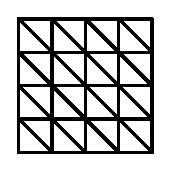
\includegraphics[width=0.6\textwidth]{./pics/triangleMesh}
											\end{tabular}
											%\caption{\footnotesize Computational domain meshed in all triangular elements.}\label{fig7: triagleMesh}
										\end{figure}
									\end{minipage}
									\begin{minipage}{0.5\textwidth}
										\begin{tabular}{c|c|c|c|c}
											\hline
											\multicolumn{5}{c}{ k = 1} \\
											\hline
											\#WG & $ Error (u_{0}) $ & $ O(u_{0}) $ & $ Error(u_{b})  $& $ O(u_{b})  $\\
											\hline
											$ 4 $ & $ 9.484e-2 $ & - & $ 8.484e-2 $ & - \\
											\hline
											$ 16 $ & $ 2.678e-3 $ & $ 1.9 $& $ 2.178e-3 $ & $ 1.9 $ \\
											\hline
											$ 64 $ & $ 5.570e-4 $ & $ 2.0 $ & $ 5.470e-4 $ & $ 1.9 $ \\
											\hline
											$ 256 $ & $ 1.437e-4 $ & $ 2.0 $ & $ 1.367e-4 $ & $ 2.0 $\\
											\hline
										\end{tabular}
									\end{minipage}
									
									%}
								\end{center} }
								\caption{Numerical results and accuracy of triangular elements.}
								\label{Tab: triangleMesh}
							\end{table}
							
							
							
							%======================================================
							
							% 		\begin{figure}[H]
							% 			\centering
							% 			\begin{tabular}{c}
							% 				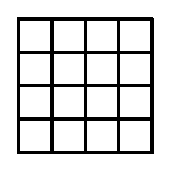
\includegraphics[width=0.3\textwidth]{./pics/quadMesh}
							% 			\end{tabular}
							% 			\caption{\footnotesize Computational domain meshed in all quadrilateral elements.}\label{fig7: quadMesh}
							% 		\end{figure}
							
							\vspace{5mm}
							\begin{table}[H]
								\small
								\vspace{-10pt}
								\setlength{\tabcolsep}{1pt} {
									\vspace{-5pt}
									\begin{center}
										%\scalebox{0.8}{
										\begin{minipage}{0.4\textwidth}
											\begin{figure}[H]
												\centering
												\begin{tabular}{c}
													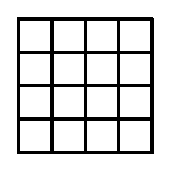
\includegraphics[width=0.6\textwidth]{./pics/quadMesh}
												\end{tabular}
												%\caption{\footnotesize Computational domain meshed in all quadrilateral elements.}\label{fig7: quadMesh}
											\end{figure}
										\end{minipage}
										\begin{minipage}{0.5\textwidth}
											\begin{tabular}{c|c|c|c|c}
												\hline
												\multicolumn{5}{c}{ k = 1} \\
												\hline
												\#WG & $ Error (u_{0}) $ & $ O(u_{0}) $ & $ Error(u_{b})  $& $ O(u_{b})  $\\
												\hline
												$ 4 $ & $ 8.368e-2 $ & - & $ 9.103e-2 $ & - \\
												\hline
												$ 16 $ & $ 1.944e-3 $ & $ 1.9 $& $ 2.058e-3 $ & $ 1.9 $ \\
												\hline
												$ 64 $ & $ 5.337e-4 $ & $ 2.0 $ & $ 5.280e-4 $ & $ 2.0 $ \\
												\hline
												$ 256 $ & $ 1.086e-4 $ & $ 2.0 $ & $ 1.451e-4 $ & $ 2.0 $\\
												\hline
											\end{tabular}
										\end{minipage}
										
										%}
									\end{center} }
									\caption{Numerical results and accuracy of quadrilateral elements.}
									\label{Tab: quadMesh}
								\end{table}
								
								After applying the BDDC scheme, we can partition the original computational domain into several non-overlapping subdomains, and, we present the scalability of parallel computing for solving Eq. (48) in Fig. \ref{fig9: time}.
								
								\vspace{5mm}
								\begin{table}[H]
									\small
									\vspace{-10pt}
									\setlength{\tabcolsep}{1pt} {
										
										\vspace{-5pt}
										\begin{center}
											%\scalebox{0.8}{
											\begin{tabular}{c|cccc|c|cccc}
												\hline
												\multirow{2}{*}{\#sub} &\multicolumn{4}{c|}{ $H/h=8$} &\multirow{2}{*}{$H/h$} &\multicolumn{4}{c}{$k=1$ and \#sub=64}\\ 
												& Cond.   & Iter. &$L_{Max}$-error & $O$& & Cond.   & Iter. &$L^2$-error & $O$ \\
												
												\hline
												$2\times 2$     & 2.281 & 8   & 8.484e-2 & - & 4   & 2.212 &11 & 2.993e-1 &- \\
												$4\times 4$     &3.922 &12 &2.1787e-2 & 1.96 & 8   & 3.069 &12 & 8.567e-2 & 1.9  \\
												$8\times 8$  & 4.895 &17 &5.4706e-3 & 1.99 & 16   & 4.143 &13 & 2.217e-2 & 2.0 \\
												$16\times 16$ &5.238&17 &1.3675e-3 & 2.00 & 32   & 5.437 &15 & 5.575e-3 & 2.0 \\
												\hline	
											\end{tabular}
											%	}
										\end{center} }
										\caption{The accuracy and convergence properties with $ \lambda = 1, \mu = 0.5 $ on quadrilateral linear elements.}
										\label{Tab:case1_PkPkPk linear}
									\end{table}
									
									%We test the performance of WG-BDDC on a computer cluster. and present the speedup figure which indicates the superlinear acceleration and good scalability. 
									
									\begin{figure}[H]
										\centering
										%	\begin{tabular}{cc}
										\includegraphics[width=0.5\textwidth]{./pics/p1time.eps} 
										%	\end{tabular}
										\caption{\footnotesize The running time .vs. number of processors.}\label{fig9: time}
									\end{figure}
									
									In this figure, we plot the average compute time of each processor for a mesh first decomposed into $ 2 \times 2 $ subdomains and then uniformly partitioned to $ 25 \times 25 $ subdomains.  the circle line represents WG-BDDC method. The total number of mesh elements remains the same. This figure indicates the reduction in compute time for increasing number of processors. 
									
									\begin{figure}[H]
										\centering
										%	\begin{tabular}{cc}
										\includegraphics[width=0.5\textwidth]{./pics/p1speed.eps}
										%	\end{tabular}
										\caption{\footnotesize The speedup .vs. number of processors.}\label{fig10: speed}
									\end{figure}
									
									
									We can see from Fig. \ref{fig10: speed} that superlinear speedup is obtained with the increasing number of subdomains. When the number of subdomains reaches $ 300 $, the highest speedup rate is achieved because it is the best ratio of global to local cost produces. The communication overhead takes the lowest portion in the total computational effort. In each local subdomain, the critical ration exists between the number of the degree of freedoms in primal space (global matrix) to these in dual space (local matrix). The costs for Cholesky elimination and the PCG  solver are $ O(n^{3}) $ and $ O(n\sqrt{(k)}) $, respectively. We can obtain significant superlinear speedup through domain decomposition. On the other hand, the growth of global matrix introduces increasing overhead. It is the main reason of the speedup curve flatting with the increasing number of processor. The main factor of the WG-BDDC method is the balance between the global matrix, the preconditioner, and the local matrices. An appropriate estimate on balancing load distributions will produce optimal performance on modern computer structure.
									
									\subsection{Locking-Free Tests}
									
									To investigate the locking-free feature of the WG-BDDC method on linear elasticity equation, we consider the exact solution given by
									
									\begin{equation}
									u = \begin{pmatrix}
									sin(2 \pi x) sin(2 \pi y) \\ cos(2 \pi x) cos(2 \pi y) \\
									\end{pmatrix} + \lambda^{-1} \begin{pmatrix}
									x \\ y
									\end{pmatrix}
									\end{equation}
									
									The locking-free feature refers to lack of constraints applied on Lame index $ \lambda $ and $ \mu $. For instance, the Poisson's ratio $ \nu $ is close to $ \frac{1}{2} $ (the material property is nearly incompressible, Lame indices $ \lambda $ is very large and $ \mu $ is $ \frac{1}{2} $) which indicates that the displacement of the exact solution must fit $ \nabla \cdot u = 0 $. This is a very challenging condition for continuous Galerkin FEM. However, this difficulty can be addressed by the WG-BDDC method. We design a series of numerical tests to explain that WG-BDDC provides good locking-free convergence.
									\vspace{5mm}
									\begin{table}[H]
										\small
										\vspace{-10pt}
										\setlength{\tabcolsep}{1pt} {
											\vspace{-5pt}
											\begin{center}
												%\scalebox{0.8}{
												\begin{tabular}{c|cccc|c|cccc}
													\hline
													\multirow{2}{*}{\#sub} &\multicolumn{4}{c|}{ $H/h=8$} &\multirow{2}{*}{$H/h$} &\multicolumn{4}{c}{$k=1$ and \#sub=64}\\ 
													& Cond.   & Iter. &$L_{Max}$-error & $O$& & Cond.   & Iter. &$L^2$-error & $O$ \\
													
													\hline
													$2\times 2$     & 2.281 & 8   & 7.522e-2 & - & 4   & 2.374 &11 & 2.535e-1 &- \\
													$4\times 4$     &3.922 &13 &2.543e-2 & 1.56 & 8   & 3.272 &12 & 8.967e-2 & 1.50  \\
													$8\times 8$  & 4.895 &16 & 7.533e-3 & 1.75 & 16   & 4.538 &13 & 2.853e-2 & 1.66 \\
													$16\times 16$ &5.238&18 & 2.017e-3 & 1.90 & 32   & 5.751 &15 & 7.834e-3 & 1.86 \\
													\hline	
												\end{tabular}
												%	}
											\end{center} }
											\caption{The accuracy and convergence properties of quadrilateral linear element, $ \lambda = 1, \mu = 0.5 $}
											\label{Tab:lockfree1}
										\end{table}
										\vspace{5mm}
										\begin{table}[ht]
											\small
											\vspace{-10pt}
											\setlength{\tabcolsep}{1pt} {
												\vspace{-5pt}
												\begin{center}
													%\scalebox{0.8}{
													\begin{tabular}{c|cccc|c|cccc}
														\hline
														\multirow{2}{*}{\#sub} &\multicolumn{4}{c|}{ $H/h=8$} &\multirow{2}{*}{$H/h$} &\multicolumn{4}{c}{$k=1$ and \#sub=64}\\ 
														& Cond.   & Iter. &$L_{Max}$-error & $O$& & Cond.   & Iter. &$L^2$-error & $O$ \\
														
														\hline
														$2\times 2$     & 2.281 & 8   & 7.523e-2 & - & 4   & 2.374 &11 & 2.535e-1 &- \\
														$4\times 4$     &3.922 &13 &2.543e-2 & 1.56 & 8   & 3.272 &12 & 8.967e-2 & 1.50  \\
														$8\times 8$  & 4.895 &16 & 7.533e-3 & 1.75 & 16   & 4.538 &13 & 2.851e-2 & 1.66 \\
														$16\times 16$ &5.238&18 & 2.017e-3 & 1.90 & 32   & 5.751 &15 & 7.834e-3 & 1.86 \\
														\hline	
													\end{tabular}
													%	}
												\end{center} }
												\caption{The accuracy and convergence properties of quadrilateral linear element, $ \lambda = 1,000, \mu = 0.5 $}
												\label{Tab:lockfree2}
											\end{table}
											
											\vspace{5mm}
											\begin{table}[ht]
												\small
												\vspace{-10pt}
												\setlength{\tabcolsep}{1pt} {
													\vspace{-5pt}
													\begin{center}`
														%\scalebox{0.8}{
														\begin{tabular}{c|cccc|c|cccc}
															\hline
															\multirow{2}{*}{\#sub} &\multicolumn{4}{c|}{ $H/h=8$} &\multirow{2}{*}{$H/h$} &\multicolumn{4}{c}{$k=1$ and \#sub=64}\\ 
															& Cond.   & Iter. &$L_{Max}$-error & $O$& & Cond.   & Iter. &$L^2$-error & $O$ \\
															
															\hline
															$2\times 2$     & 2.281 & 8   & 7.52e-2 & - & 4   & 2.374 &11 & 2.535e-1 &- \\
															$4\times 4$     &3.922 &13 &2.545e-2 & 1.56 & 8   & 3.272 &12 & 8.967e-2 & 1.50  \\
															$8\times 8$  & 4.895 &16 & 7.533e-3 & 1.75 & 16   & 4.538 &13 & 2.854e-2 & 1.66 \\
															$16\times 16$ &5.238&18 & 2.017e-3 & 1.90 & 32   & 5.751 &15 & 7.834e-3 & 1.86 \\
															\hline	
														\end{tabular}
														%	}
													\end{center} }
													\caption{The accuracy and convergence properties of quadrilateral linear element, $ \lambda = 1,000,000, \mu = 0.5 $}
													\label{Tab:lockfree3}
												\end{table}
												
												Tabless \ref{Tab:lockfree1}, \ref{Tab:lockfree2} and \ref{Tab:lockfree3} show that the order of accuracy is not affected by the values of Lame indices. The locking-free feature is inherited from the WG method and is also successfully demonstrated by the WG-BDDC scheme.
												
												%===============================================
												\section{Summary}
												In this chapter, a novel parallel computing method is presented for solving linear elasticity problems. This method integrates the newly developed weak Galerkin (WG) finite element method with the balancing domain decomposition with constraints (BDDC). The WG-BDDC method is implemented using Fortran and MPI. The WG-BDDC method is demonstrated to have optimal order of accuracy for both 2nd and 3rd order numerical discretizations. The method is also proven to have outstanding scalability with superlinear speedup when the number of processors increases to over 600 processors. The condition numbers of the Lanczos matrix from the global interface for all test cases presented in this paper are well bounded demonstrating a fast and robust convergence. The WG-BDDC method has locking-free feature. It provides accurate results for almost incompressible materials. 